%%%%%%%%%%%%%%%%%%%%%%%%%%%%%%%%%%%%%%%%%%%%%%%%%%%%%%%%%%%%%%%%%%%%%%%

% BAB 6
%%%%%%%%%%%%%%%%%%%%%%%%%%%%%%%%%%%%%%%%%%%%%%%%%%%%%%%%%%%%%%%%%%%%%%%

\mychapter{6}{BAB 6 PENGUJIAN}

\section{Pengujian Unit}

Pengujian unit dilakukan untuk memastikan hasil implementasi kode program telah
sesuai dengan hasil perancangan komponen. Komponen terkecil dari sebuah sistem
berorientasi objek adalah \emph{class} dengan \emph{testable unit} terkecilnya
adalah \emph{function} atau \emph{method}
\parencite{pressman2010software}. Pengujian unit pada \emph{class model} dan
\emph{class controller} dilakukan hingga mencapai 100\% \emph{code
  coverage}. \emph{Class} \emph{view} hanya memanggil fungsi-fungsi
yang terdapat pada \emph{class} \emph{controller} dan \emph{class model} sehingga pada
penelitian ini pengujian unit pada \emph{class} \emph{view} hanya diuji hingga
\emph{code coverage} mencapai 70\%. Metode pengujian yang digunakan adalah
\emph{white-box testing}, dan teknik pengujian yang digunakan adalah
\emph{basis path testing}. \emph{Driver} digunakan sebagai
\emph{``main program''} untuk memanggil \emph{function} yang diuji.
\emph{Stub} atau \emph{fake} digunakan agar pengujian unit benar-benar
terisolasi, bukan sebagai \emph{``stand-alone program''}.
Terdapat tiga sampel pengujian unit yang akan di paparkan pada tahapan
ini. Gambar~\ref{fig:unit-test-coverage} memperlihatkan hasil pengujian unit pada \emph{class controller}
dan \emph{class model} yang mencapai 100\% \emph{code coverage}.

\begin{figure}[tph]
  \centering
  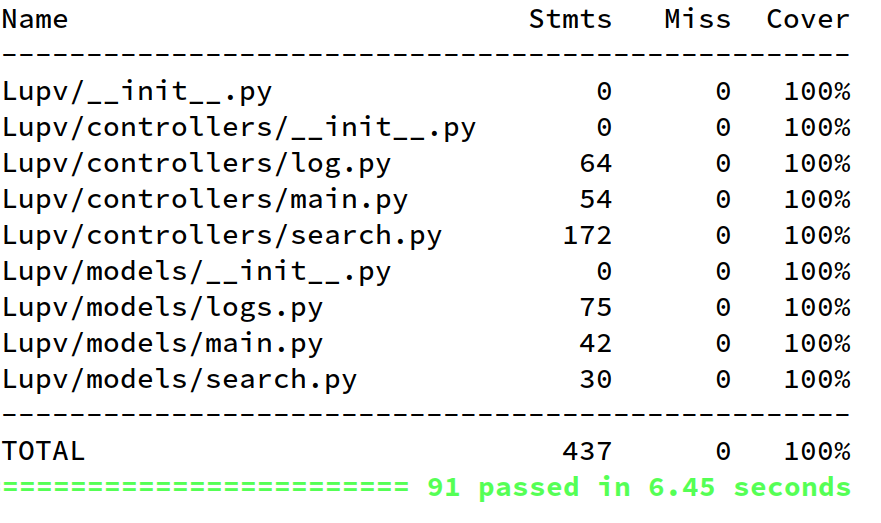
\includegraphics[width=.6\linewidth]{img/unit-test-coverage-cropped}
  \caption{Pengujian unit mencapai 100\% \emph{code coverage}}
  \label{fig:unit-test-coverage}
\end{figure}

\subsection{Pengujian Unit \emph{Class} \emph{Controller} \emph{Function} \emph{get\_all\_windows}}

Pengujian \emph{unit} dilakukan pada \emph{function}
\emph{get\_all\_windows} secara terisolasi. Maka unit lain
yang dipanggil di dalamnya akan digantikan dengan \emph{stub}.
Tabel Kode~\ref{pct:get_all_windows} dan Gambar~\ref{fg:get_all_windows}
menjelaskan \emph{basis path} dari \emph{pseudocode}
\emph{function} \emph{get\_all\_windows}. Bagian berikutnya menjelaskan
perhitungan \emph{cyclomatic complexity}, dan \emph{independent path}.
Tabel~\ref{jalur:get_all_windows} menjelaskan hasil uji dan kasus uji
dari \emph{function} \emph{get\_all\_windows}.

\par\null\par
\begin{code}
\begin{ignasicblock}[title=get\_all\_windows,minted language=text,
underlay={
  \drawline{8cm}{11.5cm}{2.5}{1}
  \drawline{8cm}{12.5cm}{3.5}{2}
  \drawline{12cm}{11.5cm}{5}{3}
  \drawline{10cm}{12.5cm}{6}{4}
  \drawbrace{12cm}{6.5}{8.5}{5}
  \drawline{8cm}{11.5cm}{10}{6}
  \drawline{8cm}{12.5cm}{11}{7}
  \drawline{8cm}{11.5cm}{12.5}{8}
 }]

START
  READ all_windows_dirty
  IF all_windows_dirty is true
    SET all_windows_dirty to split every line
    FOR each window in all_windows_dirty
      GET window_name
      SET all_windows = window_name
    ENDFOR
  ENDIF
  RETURN all_windows
END
\end{ignasicblock}
  \captionof{listing}{\emph{Pseudocode function}
    \emph{get\_all\_windows}}\label{pct:get_all_windows}
\end{code}

\begin{figure}[H]
  \centering
  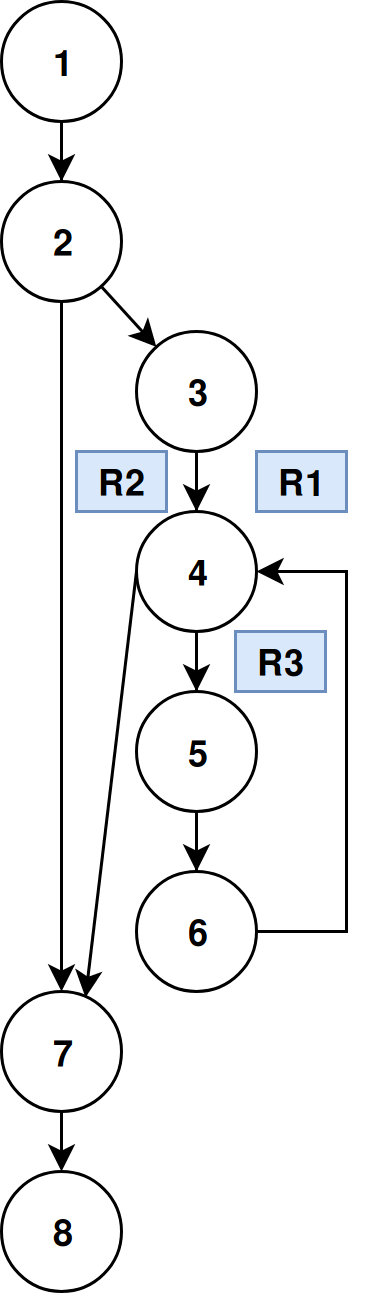
\includegraphics[width=.19\linewidth]{img/test-case/fg-get_all_windows-v2}
  \caption{\emph{Flow graph} dari \emph{pseudocode}
    \emph{get\_all\_windows}}\label{fg:get_all_windows}
\end{figure}

\noindent
\emph{Cyclomatic Complexity}

\begin{itemize}
\item V(G) = 3 \emph{regions}
\item V(G) = 9 \emph{edge} – 8 \emph{node} + 2 = 3
\item V(G) = 2 \emph{predicate node} + 1 = 3
\end{itemize}
\newpage % manual-adj
\noindent
\emph{Independent Path}

\begin{itemize}
\item Jalur 1 : 1 - 2 - 7 - 8
\item Jalur 2 : 1 - 2 - \textbf{3 - 4} - 7 - 8
\item Jalur 2 : 1 - 2 - 3 - 4 - \textbf{5 - 6} - 4 - 7 - 8
\end{itemize}

\begin{longtable}{|P{.06\textwidth}|P{.30\textwidth}|P{.30\textwidth}|P{.10\textwidth}|P{.08\textwidth}|}
  \caption{Kasus uji dan hasil uji \emph{function get\_all\_windows}}\label{jalur:get_all_windows}\\\hline
  \textbf{Jalur} & \textbf{Prosedur Uji} & \textbf{\emph{Expected Result}} & \textbf{\emph{Result}} & \textbf{Status} \\\hline
  %
  1 & 1) \emph{Set variable window\_title} dengan nilai ``None''.\par\null\par
      2) \emph{Class Driver TestController} memanggil \emph{function get\_all\_windows}
                                         & \emph{Return value} \emph{function get\_all\_windows} bernilai
                                           ``\texttt{""}''. & \emph{As expected} & Valid \\\hline
                                           %
  2 & 1) \emph{Set variable window\_title} dengan nilai ``\texttt{""}''.\par\null\par
      2) \emph{Class Driver TestController} memanggil \emph{function get\_all\_windows}.
                                         & \emph{Return value} \emph{function get\_all\_windows} bernilai
                                           ``\texttt{""}''. & \emph{As expected} & Valid \\\hline
                                           %
  3 & 1) \emph{Set variable window\_title} dengan nilai ``b\texttt{"}0x006000ab  0 machine-name
      foo\_window\_title \texttt{"}''.\par\null\par
      2) \emph{Class Driver TestController} memanggil \emph{function get\_all\_windows}.
                                         & \emph{Return value} \emph{function get\_all\_windows} bernilai
                                           ``foo\_window\_title'' & \emph{As expected} & Valid \\\hline
                                           %
  %
\end{longtable}

Pengujian unit yang dilakukan pada \emph{function} \emph{get\_all\_windows}
menghasilkan perhitungan \emph{cyclomatic complexity} dengan nilai 3 sehingga
memiliki 3 \emph{independent path} yang harus diuji. Hasil pengujian 3
\emph{path} yang dipaparkan pada Tabel~\ref{jalur:get_all_windows} bernilai valid.

\subsection{Pengujian Unit \emph{Class} \emph{LogController}
  \emph{Function} \emph{populate\_logs}}

Pengujian \emph{unit} dilakukan pada \emph{function}
\emph{populate\_logs} secara terisolasi. Maka \emph{function
  student\_record}, \emph{function is\_exist} pada unit \emph{LogModel},
dan \emph{function relativize\_datetime} pada unit
\emph{MainController} yang dipanggil di dalamnya akan digantikan
dengan \emph{stub}. Tabel Kode~\ref{pct:populate_logs} dan
Gambar~\ref{fg:populate_logs} menjelaskan \emph{basis path} dari
\emph{pseudocode} \emph{function} \emph{populate\_logs}. Bagian
berikutnya menjelaskan perhitungan \emph{cyclomatic complexity} dan
\emph{independent path}. Tabel~\ref{jalur:populate_logs} menjelaskan
hasil uji dan kasus uji dari \emph{function} \emph{populate\_logs}.

\par\null\par
\begin{code}
\begin{ignasicblock}[title=populate\_logs,minted language=text,
underlay={
  \drawline{10cm}{12cm}{2.5}{1}
  \drawline{9cm}{12.5cm}{5}{2}
  \drawbrace{12cm}{5.5}{12.5}{3}
  \drawline{10cm}{12.5cm}{13.5}{4}
  \drawline{10.5cm}{12cm}{16}{5}
  \drawbrace{12cm}{16.5}{18.7}{6}
  \drawline{6.5cm}{12.8cm}{19.6}{7}
  \drawline{6.5cm}{12cm}{21}{8}
  \drawline{6.5cm}{12.8cm}{22}{9}
  \drawbrace{12cm}{23}{26}{10}
 }]

START
  CALL log_model RETURNING student_records

  FOR each record in student_records
    CALL main_ctrl with relativize_datetime \
                         RETURNING relative_time
    GET time
    GET sha
    SET insetion to 0
    SET deletion to 0
    IF selected_file is true
      IF CALL log_model with is_exist \
                             RETURNING true
        GET insertion
        GET deletion
      ENDIF
    ENDIF
  ENDFOR
  SET log to (relative_time, time, sha,
                   insertion, deletion)
  RETURN log
END
\end{ignasicblock}
  \captionof{listing}{\emph{Pseudocode function}
    \emph{populate\_logs}}\label{pct:populate_logs}
\end{code}

\begin{figure}[H]
  \centering
  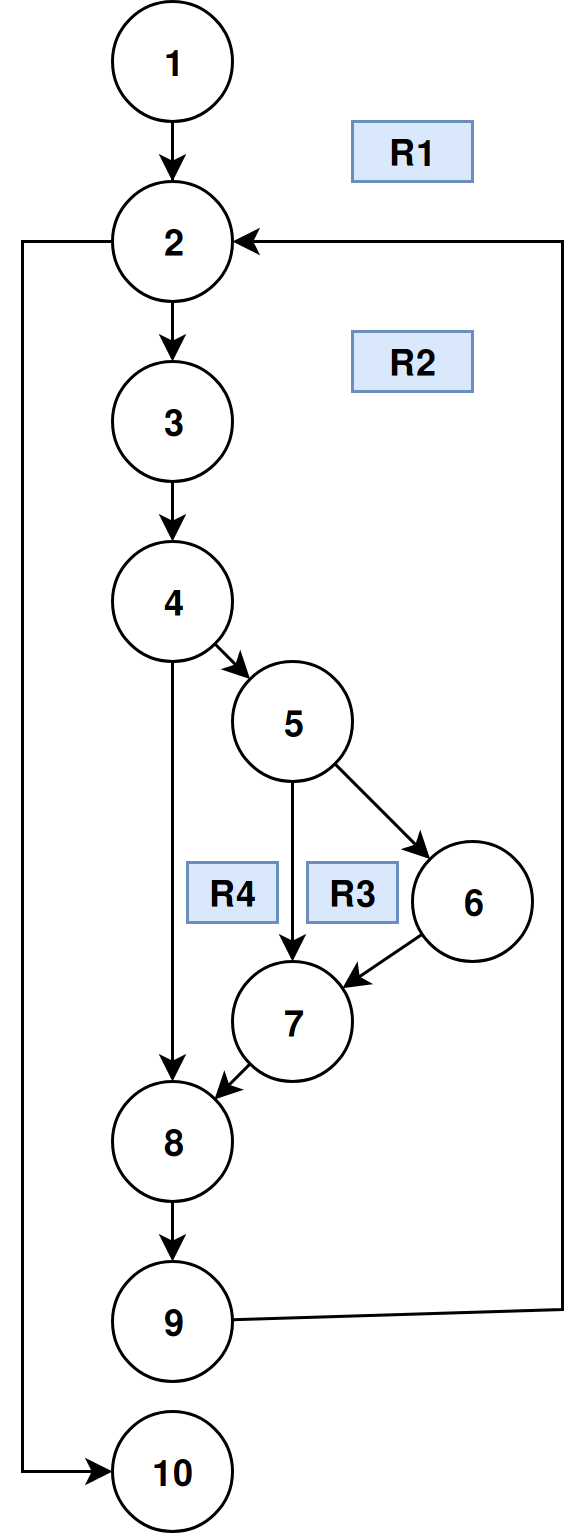
\includegraphics[width=.3\linewidth]{img/test-case/populate-logs}
  \caption{\emph{Flow graph} dari \emph{pseudocode}
    \emph{pupoulate\_logs}}\label{fg:populate_logs}
\end{figure}

\noindent
\emph{Cyclomatic Complexity}

\begin{itemize}
\item V(G) = 4 \emph{regions}
\item V(G) = 12 \emph{edge} – 10 \emph{node} + 2 = 4
\item V(G) = 3 \emph{predicate node} + 1 = 4
\end{itemize}

\noindent
\emph{Independent Path}

\begin{itemize}
\item Jalur 1: 1 - 2 - 10
\item Jalur 2: 1 - 2 - \textbf{3 - 4 - 8 - 9} - 2 - 10
\item Jalur 3: 1 - 2 - 3 - 4 - \textbf{5 - 7} - 8 - 9 - 2 - 10
\item Jalur 4: 1 - 2 - 3 - 4 - 5 - \textbf{6} - 7 - 8 - 9 - 2 - 10
\end{itemize}
\newpage % manual-adj
\begin{longtable}{|P{.06\textwidth}|P{.30\textwidth}|P{.30\textwidth}|P{.10\textwidth}|P{.08\textwidth}|}
  \caption{Kasus uji dan hasil uji \emph{function populate\_logs}} \label{jalur:populate_logs}\\
  \hline
  \textbf{Jalur} & \textbf{Prosedur Uji} & \textbf{\emph{Expected Result}} & \textbf{\emph{Result}} & \textbf{Status} \\\hline
  %
  1 & 1) \emph{Set variable student\_records} dengan nilai ``[]''.\par\null\par
      2) \emph{Class Driver TestLogController} memanggil \emph{function populate\_logs}.
                                         & \emph{Return value} \emph{function populate\_logs} bernilai
                                           ``[]''. & \emph{As expected} & Valid \\\hline
                                           %
  2 & \emph{Class Driver TestLogController} memanggil \emph{function populate\_logs} tanpa \emph{argument}.
                                         & \emph{Return value} \emph{function populate\_logs} bernilai data
                                           rekaman tanpa nilai baris yang ditambah dan dihapus.
                                                                           & \emph{As expected} & Valid \\\hline
                                           %
  3 & \emph{Class Driver TestLogController} memanggil \emph{function populate\_logs} dengan \emph{argument}
      ``selected\_file=\texttt{"}tugas-none.txt\texttt{"}''. & \emph{Return value} \emph{function populate\_logs} bernilai data
                                                               rekaman tanpa nilai baris yang ditambah dan dihapus.
                                                                           & \emph{As expected} & Valid \\\hline
  %
  4 & \emph{Class Driver TestLogController} memanggil \emph{function populate\_logs} dengan \emph{argument}
      ``selected\_file=\texttt{"}tugas-tif.txt\texttt{"}''. & \emph{Return value} \emph{function populate\_logs} bernilai data
                                                               rekaman dengan nilai baris yang ditambah dan dihapus.
                                                                           & \emph{As expected} & Valid \\\hline
  %
\end{longtable}

Pengujian unit yang dilakukan pada \emph{function populate\_logs}
menghasilkan perhitungan \emph{cyclomatic complexity} dengan nilai 4 sehingga
memiliki 4 \emph{independent path} yang harus diuji. Hasil pengujian 4
\emph{path} yang dipaparkan pada Tabel~\ref{jalur:populate_logs} bernilai valid.

\subsection{Pengujian Unit \emph{Class} \emph{SearchController} \emph{Function} \newline
  \emph{construct\_ed\_graph\_path}}

Pengujian \emph{unit} dilakukan pada \emph{function}
\emph{construct\_ed\_graph\_path} secara terisolasi. Maka unit
\emph{main\_model} yang dipanggil di dalamnya akan digantikan
dengan \emph{stub}. Tabel Kode~\ref{pct:construct_ed_graph_path} dan
Gambar~\ref{fg:construct_ed_graph_path} menjelaskan \emph{basis path}
dari \emph{pseudocode} \emph{function} \emph{construct\_ed\_graph\_path}. Bagian
berikutnya menjelaskan perhitungan \emph{cyclomatic complexity},
dan \emph{independent path}.  Tabel~\ref{jalur:construct_ed_graph_path} menjelaskan
hasil uji dan kasus uji dari \emph{function} \emph{construct\_ed\_graph\_path}.

\par\null\par
\begin{code}
\begin{ignasicblock}[title=construct\_ed\_graph\_path,minted language=text,
underlay={
  \drawline{10cm}{11.5cm}{2.3}{1}
  \drawline{10cm}{12.5cm}{4.5}{2}
  \drawline{10cm}{11.5cm}{6}{3}
  \drawline{11cm}{12.5cm}{8.5}{4}
  \drawline{7cm}{11.5cm}{9.8}{5}
  \drawbrace{11.5cm}{10.5}{13.5}{6}
 }]

START
  CALL main_model RETURNING record_path

  IF passed argument == 1
    SET graph_fmt to argument + ".png"
  ELSE
    SET graph_fmt to argument + "_" + ".png"
  ENDIF
  SET graph_path record_path + "lupv_notes" \
                                  + graph_fmt
  Return graph_path
END
\end{ignasicblock}
  \captionof{listing}{\emph{Pseudocode function}
    \emph{construct\_ed\_graph\_path}}\label{pct:construct_ed_graph_path}
\end{code}

\begin{figure}[H]
  \centering
  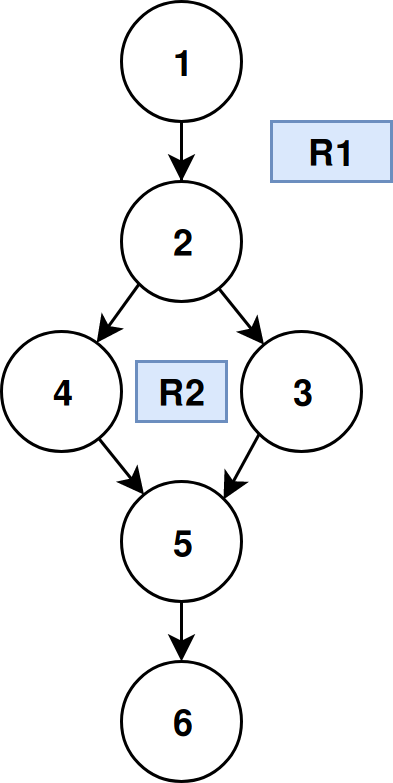
\includegraphics[width=.23\linewidth]{img/test-case/construct_ed_graph_path}
  \caption{\emph{Flow graph} dari \emph{pseudocode}
    \emph{construct\_ed\_graph\_path}}\label{fg:construct_ed_graph_path}
\end{figure}
\newpage % manual-adj
\noindent
\emph{Cyclomatic Complexity}

\begin{itemize}
\item V(G) = 2 \emph{regions}
\item V(G) = 6 \emph{edge} – 6 \emph{node} + 2 = 2
\item V(G) = 1 \emph{predicate node} + 1 = 2
\end{itemize}

\noindent
\emph{Independent Path}

\begin{itemize}
\item Jalur 1: 1 - 2 - 3 - 5 - 6
\item Jalur 2: 1 - 2 - \textbf{4} - 5 - 6
\end{itemize}

\begin{longtable}{|P{.06\textwidth}|P{.30\textwidth}|P{.30\textwidth}|P{.10\textwidth}|P{.08\textwidth}|}
  \caption{Kasus uji dan hasil uji \emph{function construct\_ed\_graph\_path}} \label{jalur:construct_ed_graph_path}\\
  \hline
  \textbf{Jalur} & \textbf{Prosedur Uji} & \textbf{\emph{Expected Result}} & \textbf{\emph{Result}} & \textbf{Status} \\\hline
  %
  1 & \emph{Class Driver TestSearchController} memanggil \emph{function construct\_ed\_graph\_path} dengan
      \emph{argument} ``ani-1111''. & \emph{Return value} \emph{function construct\_ed\_graph\_path} bernilai
                                     ``/lupv-notes/ani-1111.png''. & \emph{As expected} & Valid \\\hline
                                           %
  2 & \emph{Class Driver TestSearchController} memanggil \emph{function construct\_ed\_graph\_path} dengan
      \emph{argument} ``ani-1111", "budi-2222''. & \emph{Return value} \emph{function
                                                   construct\_ed\_graph\_path} bernilai
                                                   ``/lupv-notes/ani-1111\_budi-2222.png''. & \emph{As expected} & Valid \\\hline
  %
\end{longtable}

Pengujian unit yang dilakukan pada \emph{function construct\_ed\_graph\_path}
menghasilkan perhitungan \emph{cyclomatic complexity} dengan nilai 2 sehingga
memiliki 2 \emph{independent path} yang harus diuji. Hasil pengujian 2
\emph{path} yang dipaparkan pada Tabel~\ref{jalur:construct_ed_graph_path}
bernilai valid.


\section{Pengujian Integrasi}

Pengujian integrasi dilakukan untuk memastikan integrasi antar unit berjalan
dengan baik. Pengujian integrasi dilakukan karena terdapat kemungkinan
terjadinya masalah ketika unit dijalankan bersamaan. Sistem yang dikembangkan
menggunakan pendekatan dan pengembangan berorientasi objek sehingga pendekatan
pengujian integrasi yang digunakan adalah \emph{use-based testing}. Pengujian
integrasi diawali dari \emph{class} yang memiliki \emph{dependent class} paling
sedikit, yaitu dimulai dari \emph{class} \emph{model}, kemudian \emph{class
  controller}, dan yang terakhir adalah \emph{class} \emph{view}. Metode yang
digunakan adalah \emph{white-box testing}, dan teknik yang digunakan adalah
\emph{basis path testing}. Tujuan pengujian integrasi memastikan integrasi
komponen sistem berjalan dengan baik. Maka pada pengujian ini, \emph{function}
pada suatu \emph{class} yang memanggil \emph{function} pada \emph{class} lain
tidak digantikan dengan \emph{stub} atau \emph{fake} sebagaimana ketika pada
pengujian unit. Terdapat satu sampel pengujian integrasi yang dipaparkan, yaitu
\emph{function populate\_logs} pada \emph{class LogController} yang di dalamnya
memanggil \emph{function student\_records} dan \emph{function is\_exist} pada
\emph{class LogModel}, dan \emph{function relativize\_datetime} pada \emph{class
  MainController}.

Tabel Kode~\ref{pct:populate_logs_integration} dan
Gambar~\ref{fg:populate_logs_integration} menjelaskan \emph{basis path}
dari \emph{pseudocode} \emph{function} \emph{populate\_logs\_integration}. Bagian
berikutnya menjelaskan perhitungan \emph{cyclomatic complexity},
\emph{independent path}.  Tabel~\ref{jalur:populate_logs_integration} menjelaskan
hasil uji dan kasus uji dari \emph{function} \emph{populate\_logs}.

\begin{figure}[H] % manual-adj (figure dipindah ke depan)
  \centering
  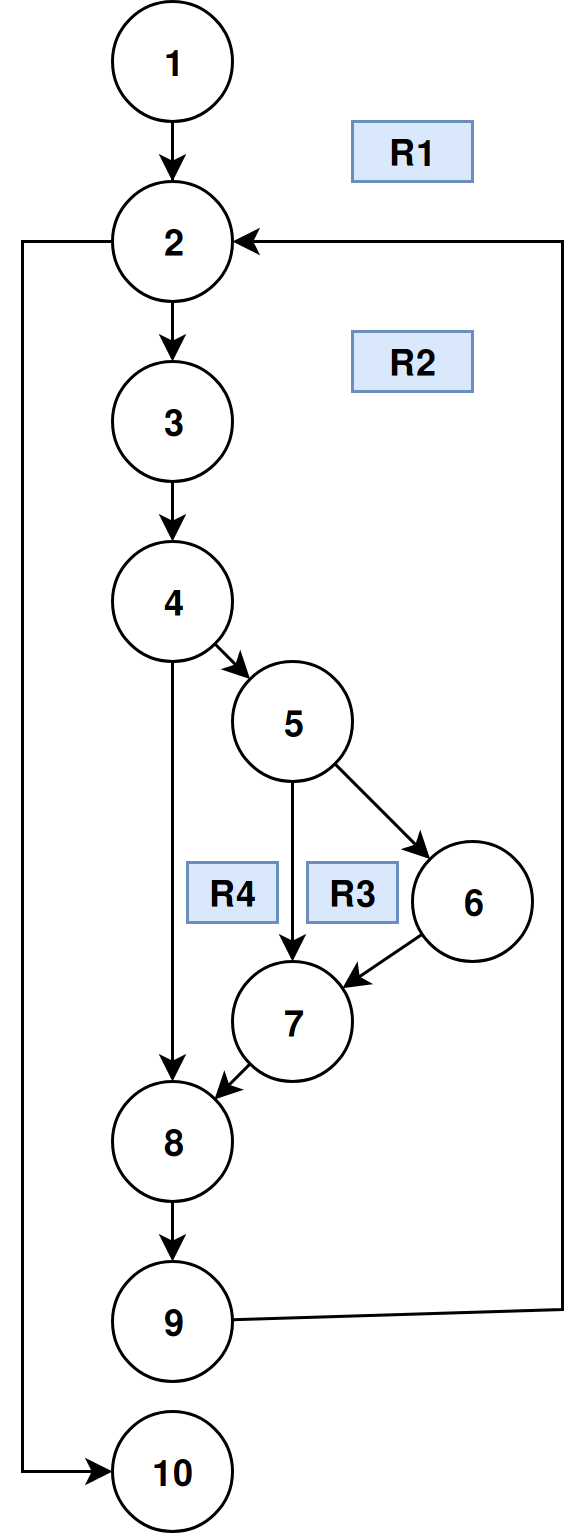
\includegraphics[width=.2\linewidth]{img/test-case/populate-logs}
  \caption{\emph{Flow graph} dari \emph{pseudocode}
    \emph{pupoulate\_logs}}\label{fg:populate_logs_integration}
\end{figure}

\par\null\par
\begin{code}
\begin{ignasicblock}[title=populate\_logs,minted language=text,
underlay={
  \drawline{10cm}{12cm}{2.5}{1}
  \drawline{9cm}{12.5cm}{5}{2}
  \drawbrace{12cm}{5.5}{12.5}{3}
  \drawline{10cm}{12.5cm}{13.5}{4}
  \drawline{10.5cm}{12cm}{16}{5}
  \drawbrace{12cm}{16.5}{18.7}{6}
  \drawline{6.5cm}{12.8cm}{19.6}{7}
  \drawline{6.5cm}{12cm}{21}{8}
  \drawline{6.5cm}{12.8cm}{22}{9}
  \drawbrace{12cm}{23}{26}{10}
 }]

START
  CALL log_model RETURNING student_records

  FOR each record in student_records
    CALL main_ctrl with relativize_datetime \
                         RETURNING relative_time
    GET time
    GET sha
    SET insetion to 0
    SET deletion to 0
    IF selected_file is true
      IF CALL log_model with is_exist \
                             RETURNING true
        GET insertion
        GET deletion
      ENDIF
    ENDIF
  ENDFOR
  SET log to (relative_time, time, sha,
                   insertion, deletion)
  RETURN log
END
\end{ignasicblock}
  \captionof{listing}{\emph{Pseudocode function}
    populate\_logs}\label{pct:populate_logs_integration}
\end{code}

\noindent
\emph{Cyclomatic Complexity}

\begin{itemize}
\item V(G) = 4 \emph{regions}
\item V(G) = 12 \emph{edge} – 10 \emph{node} + 2 = 4
\item V(G) = 3 \emph{predicate node} + 1 = 4
\end{itemize}

\noindent
\emph{Independent Path}

\begin{itemize}
\item Jalur 1: 1 - 2 - 10
\item Jalur 2: 1 - 2 - \textbf{3 - 4 - 8 - 9} - 2 - 10
\item Jalur 3: 1 - 2 - 3 - 4 - \textbf{5 - 7} - 8 - 9 - 2 - 10
\item Jalur 4: 1 - 2 - 3 - 4 - 5 - \textbf{6} - 7 - 8 - 9 - 2 - 10
\end{itemize}

\begin{longtable}{|P{.06\textwidth}|P{.30\textwidth}|P{.30\textwidth}|P{.10\textwidth}|P{.08\textwidth}|}
  \caption{Kasus uji dan hasil uji \emph{function populate\_logs}} \label{jalur:populate_logs_integration}\\
  \hline
  \textbf{Jalur} & \textbf{Prosedur Uji} & \textbf{\emph{Expected Result}} & \textbf{\emph{Result}} & \textbf{Status} \\\hline
  %
  1 & 1) \emph{Set variable student\_records} dengan nilai ``[]''.\par\null\par
      2) \emph{Class Driver TestLogController} memanggil \emph{function populate\_logs}.
                                         & \emph{Return value} \emph{function populate\_logs} bernilai
                                           ``[]''. & \emph{As expected} & Valid \\\hline
                                           %
  2 & \emph{Class Driver TestLogController} memanggil \emph{function populate\_logs} tanpa \emph{argument}.
                                         & \emph{Return value} \emph{function populate\_logs} bernilai data
                                           rekaman tanpa nilai baris yang ditambah dan dihapus.
                                                                           & \emph{As expected} & Valid \\\hline
                                           %
  3 & \emph{Class Driver TestLogController} memanggil \emph{function populate\_logs} dengan \emph{argument}
      ``selected\_file=\texttt{"}tugas-none.txt\texttt{"}''. & \emph{Return value} \emph{function populate\_logs} bernilai data
                                                               rekaman tanpa nilai baris yang ditambah dan dihapus.
                                                                           & \emph{As expected} & Valid \\\hline
  %
  4 & \emph{Class Driver TestLogController} memanggil \emph{function populate\_logs} dengan \emph{argument}
      ``selected\_file=\texttt{"}tugas-tif.txt\texttt{"}''. & \emph{Return value} \emph{function populate\_logs} bernilai data
                                                               rekaman dengan nilai baris yang ditambah dan dihapus.
                                                                           & \emph{As expected} & Valid \\\hline
  %
\end{longtable}

Pengujian integrasi yang dilakukan pada \emph{function populate\_logs}
menghasilkan perhitungan \emph{cyclomatic complexity} dengan nilai 4 sehingga
memiliki 4 \emph{independent path} yang harus diuji. Hasil pengujian 4
\emph{path} yang dipaparkan pada Tabel~\ref{jalur:populate_logs_integration} bernilai valid.

\section{Pengujian Validasi}

Pengujian validasi dilakukan untuk memastikan bahwa sistem yang
dibangun sesuai dengan seluruh skenario kebutuhan yang
didefinisikan. Pengujian validasi fokus terhadap
\emph{user-visible action} dan \emph{user-recognizable output}
dari sistem \parencite{pressman2010software}. Dalam pengujian validasi metode pengujian yang
digunakan adalah \emph{black-box testing}. Teknik yang digunakan
untuk memilih nilai masukan pada pengujian adalah teknik
\emph{boundary value analysis} dan \emph{equvalence
  partitioning}, kedua teknik tersebut digunakan untuk
menghindari \emph{rigorous testing} atau mencoba semua nilai
\emph{input}.

\subsection{Pengujian Validasi Merekam Pengerjaan Tugas}

Pengujian validasi ``Merekam Pengerjaan Tugas'' dilakukan untuk
menguji spesifikasi kebutuhan fungsional LUPR-F-01. Terdapat
tiga kasus uji pada pengujian ini. Kasus uji pertama pada
Tabel~\ref{tab:val-record-main} memastikan bahwa sistem memulai
perekaman tugas, kasus uji kedua pada
Tabel~\ref{tab:val-record-2} memastikan bahwa sistem berhenti
dan keluar, dan kasus uji ketiga pada
Tabel~\ref{tab:val-record-1} memastikan sistem menutup dialog
pemilihan direktori tugas

\begin{longtable}{|L{3cm}|L{9cm}|}
  \caption{Kasus uji dan hasil uji Merekam Pengerjaan Tugas}\label{tab:val-record-main} \\
  \hline
  %
  \textbf{Kode Kebutuhan} & LUPR-F-01 \\\hline
  %
  \textbf{Nama Kasus Uji} & Merekam Pengerjaan Tugas \\\hline
  %
  \textbf{Prosedur} & 1. Mengeklik tombol ``\emph{Start Recording}''.\par
                      2. Memilih direktori tempat tugas.\newline
                      3. Mengeklik tombol ``\emph{Choose}''.\\\hline
  %
  \textbf{\emph{Expected Result}} & Sistem memulai perekaman pengerjaan tugas dan menampilkan pesan
                                    notifikasi ``\emph{Lup is recording}'' menandakan bahwa
                                    perekaman telah dimulai. \\\hline
  %
  \textbf{\emph{Result}} & \emph{As expected} \\\hline
  %
  \textbf{Status} & Valid\\\hline
\end{longtable}

\begin{longtable}{|L{3cm}|L{9cm}|}
  \caption{Kasus uji dan hasil uji Merekam Pengerjaan Tugas alternatif 1}\label{tab:val-record-1} \\
  \hline
  %
  \textbf{Kode Kebutuhan} & LUPR-F-01 \\\hline
  %
  \textbf{Nama Kasus Uji} & Merekam Pengerjaan Tugas alternatif 1\\\hline
  %
  \textbf{Prosedur} & 1. Mengeklik tombol ``\emph{Stop and Quit}''.\\\hline
  %
  \textbf{\emph{Expected Result}} & Sistem berhenti dan keluar. \\\hline
  %
  \textbf{\emph{Result}} & \emph{As expected} \\\hline
  %
  \textbf{Status} & Valid\\\hline
\end{longtable}

\begin{longtable}{|L{3cm}|L{9cm}|}
  \caption{Kasus uji dan hasil uji Merekam Pengerjaan Tugas alternatif 2}
  \label{tab:val-record-2} \\
  \hline
  %
  \textbf{Kode Kebutuhan} & LUPR-F-01 \\\hline
  %
  \textbf{Nama Kasus Uji} & Merekam Pengerjaan Tugas alternatif 2\\\hline
  %
  \textbf{Prosedur} & 1. Mengeklik tombol ``\emph{Start Recording}''.\par
                      2. Memilih direktori tempat tugas.\newline
                      3. Mengeklik tombol ``\emph{Cancel}''.\\\hline
                      %
  %
  \textbf{\emph{Expected Result}} & Sistem menutup dialog pemilihan direktori tugas. \\\hline
  %
  \textbf{\emph{Result}} & \emph{As expected} \\\hline
  %
  \textbf{Status} & Valid\\\hline
\end{longtable}

Hasil pengujian validasi ``Merekam Pengerjaan Tugas'' yang memiliki 3 kasus uji
yaitu pada Tabel~\ref{tab:val-record-main}, Tabel~\ref{tab:val-record-1}, dan
Tabel~\ref{tab:val-record-2} menghasilkan nilai valid. Maka dapat dipastikan
fungsionalitas ``Merekam Pengerjaan Tugas'' sudah sesuai dengan kebutuhan yang
didefinisikan.

\subsection{Pengujian Validasi Mengubah Interval Rekaman}

Pengujian validasi ``Mengubah Interval Rekaman'' membutuhkan
\emph{range} nilai yang harus dimasukkan penguji untuk melakukan
validasi. Agar terhindar dari \emph{rigorous testing} digunakan
teknik \emph{boundary value analysis} dan \emph{equvalence
  partitioning} untuk menentukan nilai yang dimasukkan dalam
pengujian. Nilai yang valid adalah semua bilangan bulat di atas 0.\newline

\noindent
Kasus uji yang didapatkan dengan teknik \emph{equivalence partitioning}:

\begin{enumerate}
\item Kasus uji \emph{valid input}: ``2''
\item Kasus uji \emph{invalid input}: ``kolom kosong''
\end{enumerate}

\noindent
Kasus uji yang didapatkan dengan teknik \emph{boundary value analysis}:

\begin{enumerate}
\item Kasus uji \emph{valid input}: ``1''
\item Kasus uji \emph{invalid input}: ``0''
\end{enumerate}

Terdapat dua kasus uji dengan teknik \emph{equivalence partitioning},
pertama pada Tabel~\ref{tab:val-set-interval-ep-1} dengan nilai \emph{input} ``2''
memastikan bahwa sistem berhasil mengubah nilai interval,
kedua pada Tabel~\ref{tab:val-set-interval-ep-2} dengan mengosongkan
kolom memastikan bahwa sistem menampilkan pesan peringatan. Teknik
\emph{boundary value analysis} juga menghasilkan dua kasus uji.
Pertama pada Tabel~\ref{tab:val-set-interval-bva-1} dengan nilai \emph{input}
``1'' memastikan bahwa sistem berhasil mengubah nilai interval, kasus
uji kedua pada Tabel~\ref{tab:val-set-interval-bva-2} dengan nilai \emph{input}
``0'' memastikan bahwa sistem menampilkan pesan peringatan.

\begin{longtable}{|L{3cm}|L{9cm}|}
  \caption{Kasus uji dan hasil uji Mengubah Interval Rekaman
  (\emph{valid input equivalence partitioning})}\label{tab:val-set-interval-ep-1} \\
  \hline
  %
  \textbf{Kode Kebutuhan} & LUPR-F-02 \\\hline
  %
  \textbf{Nama Kasus Uji} & Mengubah Interval Rekaman \\\hline
  %
  \textbf{Prosedur} & 1. Mengeklik tombol ``\emph{Set Interval}''.\newline
                      2. Mengisi nilai 2 pada dialog interval.\newline
                      3. Mengeklik tombol ``\emph{Apply}''.\\\hline
  %
  \textbf{\emph{Expected Result}} & Sistem mengubah nilai interval rekaman dan menampilkan pesan
                                    notifikasi ``\emph{Interval changed to 2}''. \\\hline
  %
  \textbf{\emph{Result}} & \emph{As expected} \\\hline
  %
  \textbf{Status} & Valid\\\hline
\end{longtable}

\begin{longtable}{|L{3cm}|L{9cm}|}
  \caption{Kasus uji dan hasil uji Mengubah Interval Rekaman alternatif
  1 (\emph{invalid input equivalence partitioning})}\label{tab:val-set-interval-ep-2} \\
  \hline
  %
  \textbf{Kode Kebutuhan} & LUPR-F-02 \\\hline
  %
  \textbf{Nama Kasus Uji} & Mengubah Interval Rekaman alternatif 1\\\hline
  %
  \textbf{Prosedur} & 1. Mengeklik tombol ``\emph{Set Interval}''.\newline
                      2. Mengosongkan dialog interval.\newline
                      3. Mengeklik tombol ``\emph{Apply}''.\\\hline
  %
  \textbf{\emph{Expected Result}} & Sistem menampilkan pesan peringatan ``\emph{Interval must higher
                                    than 0}''. Nilai interval
                                    rekaman tidak dirubah. \\\hline
  %
  \textbf{\emph{Result}} & \emph{As expected} \\\hline
  %
  \textbf{Status} & Valid\\\hline
\end{longtable}
\newpage % manual-adj
\begin{longtable}{|L{3cm}|L{9cm}|}
  \caption{Kasus uji dan hasil uji Mengubah Interval Rekaman
  (\emph{valid input boundary value analysis})}\label{tab:val-set-interval-bva-1} \\
  \hline
  %
  \textbf{Kode Kebutuhan} & LUPR-F-02 \\\hline
  %
  \textbf{Nama Kasus Uji} & Mengubah Interval Rekaman \\\hline
  %
  \textbf{Prosedur} & 1. Mengeklik tombol ``\emph{Set Interval}''.\newline
                      2. Mengisi nilai 1 pada dialog interval.\newline
                      3. Mengeklik tombol ``\emph{Apply}''.\\\hline
  %
  \textbf{\emph{Expected Result}} & Sistem mengubah nilai interval rekaman dan menampilkan pesan
                                    notifikasi ``\emph{Interval changed to 1}''. \\\hline
  %
  \textbf{\emph{Result}} & \emph{As expected} \\\hline
  %
  \textbf{Status} & Valid\\\hline
\end{longtable}

\begin{longtable}{|L{3cm}|L{9cm}|}
  \caption{Kasus uji dan hasil uji Mengubah Interval Rekaman alternatif
  1 (\emph{invalid input boundary value analysis} )}\label{tab:val-set-interval-bva-2} \\
  \hline
  %
  \textbf{Kode Kebutuhan} & LUPR-F-02 \\\hline
  %
  \textbf{Nama Kasus Uji} & Mengubah Interval Rekaman alternatif 1\\\hline
  %
  \textbf{Prosedur} & 1. Mengeklik tombol ``\emph{Set Interval}''.\newline
                      2. Mengisi nilai 0 pada dialog interval.\newline
                      3. Mengeklik tombol ``\emph{Apply}''.\\\hline
  %
  \textbf{\emph{Expected Result}} & Sistem menampilkan pesan peringatan ``\emph{Interval must higher
                                    than 0}''. Nilai interval
                                    rekaman tidak dirubah. \\\hline
  %
  \textbf{\emph{Result}} & \emph{As expected} \\\hline
  %
  \textbf{Status} & Valid\\\hline
\end{longtable}

Hasil pengujian validasi ``Mengubah Interval Rekaman'' yang memiliki 2 kasus uji
dari teknik \emph{equivalence partitioning} pada
Tabel~\ref{tab:val-set-interval-ep-1} dan Tabel~\ref{tab:val-set-interval-ep-2}
serta 2 kasus uji dengan teknik \emph{boundary value analysis} pada
Tabel~\ref{tab:val-set-interval-bva-1} dan
Tabel~\ref{tab:val-set-interval-bva-2} menghasilkan nilai valid. Maka dapat
dipastikan fungsionalitas ``Mengubah Interval Rekaman'' sudah sesuai dengan
kebutuhan yang didefinisikan.

\subsection{Pengujian Validasi Melihat Seluruh Daftar Rekaman}

Pengujian validasi ``Melihat Seluruh Daftar Rekaman'' dilakukan
untuk menguji spesifikasi kebutuhan fungsional
LUPV-F-01. Terdapat tiga kasus uji pada pengujian ini. Kasus
uji pertama pada Tabel~\ref{tab:val-dashboard-main} memastikan
bahwa sistem menampilkan seluruh daftar rekaman mahasiswa,
Tabel~\ref{tab:val-dashboard-1} memastikan bahwa sistem menutup
dialog pemilihan rekaman, dan kasus uji ketiga pada
Tabel~\ref{tab:val-dashboard-2} memastikan sistem menampilkan
pesan peringatan bahwa direktori berkas tidak valid.

\begin{longtable}{|L{3cm}|L{9cm}|}
  \caption{Kasus uji dan hasil uji Melihat Seluruh Daftar Rekaman}\label{tab:val-dashboard-main} \\
  \hline
  %
  \textbf{Kode Kebutuhan} & LUPV-F-01 \\\hline
  %
  \textbf{Nama Kasus Uji} & Melihat Seluruh Daftar Rekaman \\\hline
  %
  \textbf{Prosedur} & 1. Mengeklik tombol ``\emph{Open Records}''.\newline
                      2. Memilih direktori rekaman. \newline
                      3. Mengeklik tombol ``\emph{Choose}''.\\\hline
  %
  \textbf{\emph{Expected Result}} & Sistem menampilkan seluruh daftar rekaman mahasiswa, dengan data
                                    yang ditampilkan meliputi nama, nim, total rekaman, waktu rekaman
                                    awal, waktu rekaman akhir dan durasi pengerjaan.\\\hline
  %
  \textbf{\emph{Result}} & \emph{As expected} \\\hline
  %
  \textbf{Status} & Valid\\\hline
\end{longtable}

\begin{longtable}{|L{3cm}|L{9cm}|}
  \caption{Kasus uji dan hasil uji Melihat Seluruh Daftar Rekaman alternatif 1}\label{tab:val-dashboard-1} \\
  \hline
  %
  \textbf{Kode Kebutuhan} & LUPV-F-01 \\\hline
  %
  \textbf{Nama Kasus Uji} & Melihat Seluruh Daftar Rekaman alternatif 1 \\\hline
  %
  \textbf{Prosedur} & 1. Mengeklik tombol ``\emph{Open Records}''.\newline
                      2. Memilih direktori rekaman. \newline
                      3. Mengeklik tombol ``\emph{Cancel}''.\\\hline
  %
  \textbf{\emph{Expected Result}} & Sistem menutup dialog pemilihan rekaman dan berkas rekaman tidak
                                    dibuka.\\\hline
  %
  \textbf{\emph{Result}} & \emph{As expected} \\\hline
  %
  \textbf{Status} & Valid\\\hline
\end{longtable}

\begin{longtable}{|L{3cm}|L{9cm}|}
  \caption{Kasus uji dan hasil uji Melihat Seluruh Daftar Rekaman alternatif 2}\label{tab:val-dashboard-2} \\
  \hline
  %
  \textbf{Kode Kebutuhan} & LUPV-F-01 \\\hline
  %
  \textbf{Nama Kasus Uji} & Melihat Seluruh Daftar Rekaman alternatif 2\\\hline
  %
  \textbf{Prosedur} & 1. Mengeklik tombol ``\emph{Open Records}''.\newline
                      2. Memilih direktori rekaman yang tidak valid, yaitu tidak sesuai dengan
                      spesifikasi kebutuhan kode LUPV-F-01-02 dan LUPV-F-01-03.\newline
                      3. Mengeklik tombol ``\emph{Choose}''.\\\hline
  %
  \textbf{\emph{Expected Result}} & Sistem menampilkan pesan peringatan ``\emph{Not a
                                    valid Task directory (baris baru) Contains invalid Task:
                                    <<direktori yang tidak valid>>}'' dan berkas rekaman tidak
                                    dibuka.\\\hline
  %
  \textbf{\emph{Result}} & \emph{As expected} \\\hline
  %
  \textbf{Status} & Valid\\\hline
\end{longtable}

Hasil pengujian validasi ``Melihat Seluruh Daftar Rekaman'' yang memiliki 3 kasus uji
yaitu pada Tabel~\ref{tab:val-dashboard-main}, Tabel~\ref{tab:val-dashboard-1}, dan
Tabel~\ref{tab:val-dashboard-2} menghasilkan nilai valid. Maka dapat dipastikan
fungsionalitas ``Melihat Seluruh Daftar Rekaman'' sudah sesuai dengan kebutuhan yang
didefinisikan.

\subsection{Pengujian Validasi Melihat Hasil Rekaman}

Pengujian validasi ``Melihat Hasil Rekaman'' dilakukan untuk
menguji spesifikasi kebutuhan fungsional LUPV-F-02. Terdapat
empat kasus uji pada pengujian ini. Kasus uji pertama pada
Tabel~\ref{tab:show-records-main} memastikan bahwa sistem
menampilkan hasil rekaman, Tabel~\ref{tab:show-records-1}
memastikan bahwa sistem menampilkan pesan informasi bahwa tidak
ada berkas yang dipilih, kasus uji ketiga pada
Tabel~\ref{tab:show-records-2} memastikan bahwa sistem
menampilkan pesan informasi bahwa tidak ada rekaman pada suatu
berkas, dan kasus uji keempat pada
Tabel~\ref{tab:show-records-3} memastikan bahwa sistem
menampilkan pesan peringatan untuk memilih berkas tugas.

\begin{longtable}{|L{3cm}|L{9cm}|}
  \caption{Kasus uji dan hasil uji Melihat Hasil Rekaman}\label{tab:show-records-main} \\
  \hline
  %
  \textbf{Kode Kebutuhan} & LUPV-F-02 \\\hline
  %
  \textbf{Nama Kasus Uji} & Melihat Hasil Rekaman \\\hline
  %
  \textbf{Prosedur} & 1. Mengeklik \emph{clickable} baris mahasiswa pada seluruh daftar rekaman. \newline
                      2. Mengeklik \emph{clickable} baris daftar rekaman. \newline
                      3. Memilih nama berkas pada tombol \emph{combo box}
                      ``\emph{Filename}''.\newline
                      4. Memilih tombol ``\emph{Line Insertion and Deletion}''.\newline
                      5. Memilih tombol ``\emph{Show Mode}'' dan ``\emph{Diff Mode}''.\\\hline
  %
  \textbf{\emph{Expected Result}} & Sistem Menampilkan hasil rekaman dan
                                    mengalihkan tampilan berkas antar mode ``\emph{show}'' dan
                                    ``\emph{diff}''. Hasil rekaman yang
                                    ditampilkan terdiri dari
                                    tanggal dan waktu rekaman, isi perubahan
                                    berkas, jumlah baris yang dihapus dan ditambah
                                    pada berkas, alamat \emph{IP}, seluruh
                                    \emph{window}, \emph{window} yang aktif,
                                    nama \emph{login}, dan nama piranti.\\\hline
                                    %
  \textbf{\emph{Result}} & \emph{As expected} \\\hline
  %
  \textbf{Status} & Valid\\\hline
\end{longtable}

\begin{longtable}{|L{3cm}|L{9cm}|}
  \caption{Kasus uji dan hasil uji Melihat Hasil Rekaman alternatif 1}\label{tab:show-records-1} \\
  \hline
  %
  \textbf{Kode Kebutuhan} & LUPV-F-02 \\\hline
  %
  \textbf{Nama Kasus Uji} & Melihat Hasil Rekaman alternatif 1 \\\hline
  %
  \textbf{Prosedur} & 1. Mengeklik \emph{clickable} baris mahasiswa pada seluruh daftar rekaman. \newline
                      2. Mengeklik \emph{clickable} baris daftar rekaman.\\\hline
  %
  \textbf{\emph{Expected Result}} & Sistem menampilkan pesan informasi pada berkas rekaman dengan
                                    pesan ``\emph{No file selected, please select one}''.\\\hline
  %
  \textbf{\emph{Result}} & \emph{As expected} \\\hline
  %
  \textbf{Status} & Valid\\\hline
\end{longtable}

\begin{longtable}{|L{3cm}|L{9cm}|}
  \caption{Kasus uji dan hasil uji Melihat Hasil Rekaman alternatif 2}\label{tab:show-records-2} \\
  \hline
  %
  \textbf{Kode Kebutuhan} & LUPV-F-02 \\\hline
  %
  \textbf{Nama Kasus Uji} & Melihat Hasil Rekaman alternatif 2\\\hline
  %
  \textbf{Prosedur} & 1. Mengeklik \emph{clickable} baris mahasiswa pada seluruh daftar rekaman. \newline
                      2. Mengeklik \emph{clickable} baris daftar rekaman. \newline
                      3. Memilih nama berkas pada tombol \emph{combo box}
                      ``\emph{Filename}''.\\\hline
  %
  \textbf{\emph{Expected Result}} & Sistem menampilkan pesan informasi pada berkas rekaman dengan
                                    pesan ``\emph{No availiable record for «nama berkas» in this
                                    period}''.\\\hline
  %
  \textbf{\emph{Result}} & \emph{As expected} \\\hline
  %
  \textbf{Status} & Valid\\\hline
\end{longtable}

\begin{longtable}{|L{3cm}|L{9cm}|}
  \caption{Kasus uji dan hasil uji Melihat Hasil Rekaman alternatif 3}\label{tab:show-records-3} \\
  \hline
  %
  \textbf{Kode Kebutuhan} & LUPV-F-02 \\\hline
  %
  \textbf{Nama Kasus Uji} & Melihat Hasil Rekaman alternatif 3\\\hline
  %
  \textbf{Prosedur} & 1. Mengeklik \emph{clickable} baris mahasiswa pada seluruh daftar rekaman. \newline
                      2. Mengeklik \emph{clickable} baris daftar rekaman. \newline
                      3. Memilih tombol ``\emph{Line Insertion and Deletion}''. \\\hline
                      %
  %
  \textbf{\emph{Expected Result}} & Sistem menampilkan pesan peringatan ``\emph{Please
                                    choose a file}''.\\\hline
  %
  \textbf{\emph{Result}} & \emph{As expected} \\\hline
  %
  \textbf{Status} & Valid\\\hline
\end{longtable}

Hasil pengujian validasi ``Melihat Hasil Rekaman'' yang memiliki 4 kasus uji
yaitu pada Tabel~\ref{tab:show-records-main}, Tabel~\ref{tab:show-records-1},
Tabel~\ref{tab:show-records-2} dan Tabel~\ref{tab:show-records-3} menghasilkan
nilai valid. Maka dapat dipastikan fungsionalitas ``Melihat Hasil Rekaman''
sudah sesuai dengan kebutuhan yang didefinisikan.

\subsection{Pengujian Validasi Mencari Tersangka}

Pengujian validasi ``Mencari Tersangka'' membutuhkan
\emph{range} nilai yang harus dimasukkan penguji untuk melakukan
validasi. Agar terhindar dari \emph{rigorous testing}, digunakan
teknik \emph{boundary value analysis} dan \emph{equvalence
  partitioning} untuk menentukan nilai \emph{input} yang dimasukkan dalam
pengujian. Nilai yang valid adalah semua bilangan bulat di atas 0.\newline

\noindent
Kasus uji yang didapatkan dengan teknik \emph{equivalence partitioning}:

\begin{itemize}
\item Kasus uji \emph{valid input}: ``2''
\item Kasus uji \emph{invalid input}: ``kolom kosong''
\end{itemize}

\noindent
Kasus uji yang didapatkan dengan teknik \emph{boundary value analysis}:

\begin{itemize}
\item Kasus uji \emph{valid input}: ``1''
\item Kasus uji \emph{invalid input}: ``0''
\end{itemize}

Terdapat dua kasus uji dengan teknik \emph{equivalence partitioning},
pertama pada Tabel~\ref{tab:search-suspect-ep-1} dengan nilai \emph{input} ``2''
memastikan bahwa sistem menampilkan hasil pencarian, kasus uji
kedua pada Tabel~\ref{tab:search-suspect-ep-2} dengan mengosongkan
kolom memastikan bahwa sistem menampilkan pesan peringatan.
Teknik \emph{boundary value analysis} juga menghasilkan dua kasus uji.
Pertama pada Tabel~\ref{tab:search-suspect-bva-1} dengan nilai \emph{input}
``1'' memastikan bahwa sistem menampilkan hasil pencarian, kasus
uji kedua pada Tabel~\ref{tab:search-suspect-bva-2} dengan nilai \emph{input}
``0'' memastikan bahwa sistem menampilkan pesan peringatan.

Dua kasus uji lainnya terdapat pada Tabel~\ref{tab:search-suspect-2}
untuk memastikan bahwa sistem menampilkan informasi jika tidak ada
\emph{suspect} yang ditemukan, dan pada
Tabel~\ref{tab:search-suspect-3} untuk memastikan bahwa sistem
menampilkan pesan peringatan jika tidak ada berkas yang dipilih.

\begin{longtable}{|L{3cm}|L{9cm}|}
  \caption{Kasus uji dan hasil uji Mencari Tersangka (\emph{valid input
  equivalence partitioning})}\label{tab:search-suspect-ep-1} \\
  \hline
  %
  \textbf{Kode Kebutuhan} & LUPV-F-03 \\\hline
  %
  \textbf{Nama Kasus Uji} & Mencari Tersangka\\\hline
  %
  \textbf{Prosedur} & 1. Memilih nama berkas dari tombol \emph{combo box}
                      ``\emph{Filename}''.\newline
                      2. Mengisi nilai 2 pada kolom ``\emph{Insertion
                      Limit}''. \newline
                      3. Mengeklik tombol ``\emph{Search}''.\\\hline
                      %
  %
  \textbf{\emph{Expected Result}} & Sistem menampilkan hasil pencarian tersangka.\\\hline
  %
  \textbf{\emph{Result}} & \emph{As expected} \\\hline
  %
  \textbf{Status} & Valid\\\hline
\end{longtable}

\begin{longtable}{|L{3cm}|L{9cm}|}
  \caption{Kasus uji dan hasil uji Mencari Tersangka alternatif 1
  (\emph{invalid input equivalence partitioning})}\label{tab:search-suspect-ep-2} \\
  \hline
  %
  \textbf{Kode Kebutuhan} & LUPV-F-03 \\\hline
  %
  \textbf{Nama Kasus Uji} & Mencari Tersangka alternatif 2\\\hline
  %
  \textbf{Prosedur} & 1. Memilih nama berkas dari tombol \emph{combo box}
                      ``\emph{Filename}''.\newline
                      2. Mengosongkan  kolom ``\emph{Insertion
                      Limit}''. \newline
                      3. Mengeklik tombol ``\emph{Search}''.\\\hline

  %
  \textbf{\emph{Expected Result}} & Sistem menampilkan pesan peringatan ``\emph{Please set limit
                                    higher than 0. Above 10 is recommended}''.\\\hline
  %
  \textbf{\emph{Result}} & \emph{As expected} \\\hline
  %
  \textbf{Status} & Valid\\\hline
\end{longtable}

\begin{longtable}{|L{3cm}|L{9cm}|}
  \caption{Kasus uji dan hasil uji Mencari Tersangka (\emph{valid input boundary
  value analysis})}\label{tab:search-suspect-bva-1} \\
  \hline
  %
  \textbf{Kode Kebutuhan} & LUPV-F-03 \\\hline
  %
  \textbf{Nama Kasus Uji} & Mencari Tersangka\\\hline
  %
  \textbf{Prosedur} & 1. Memilih nama berkas dari tombol \emph{combo box}
                      ``\emph{Filename}''.\newline
                      2. Mengisi nilai 1 pada kolom ``\emph{Insertion
                      Limit}''. \newline
                      3. Mengeklik tombol ``\emph{Search}''.\\\hline
                      %
  %
  \textbf{\emph{Expected Result}} & Sistem menampilkan hasil pencarian tersangka.\\\hline
  %
  \textbf{\emph{Result}} & \emph{As expected} \\\hline
  %
  \textbf{Status} & Valid\\\hline
\end{longtable}

\begin{longtable}{|L{3cm}|L{9cm}|}
  \caption{Kasus uji dan hasil uji Mencari Tersangka alternatif 1
  (\emph{invalid input boundary value analysis})}\label{tab:search-suspect-bva-2} \\
  \hline
  %
  \textbf{Kode Kebutuhan} & LUPV-F-03 \\\hline
  %
  \textbf{Nama Kasus Uji} & Mencari Tersangka alternatif 2\\\hline
  %
  \textbf{Prosedur} & 1. Memilih nama berkas dari tombol \emph{combo box}
                      ``\emph{Filename}''.\newline
                      2. Mengisi nilai 0 pada kolom ``\emph{Insertion
                      Limit}''. \newline
                      3. Mengeklik tombol ``\emph{Search}''.\\\hline

  %
  \textbf{\emph{Expected Result}} & Sistem menampilkan pesan peringatan ``\emph{Please set limit
                                    higher than 0. Above 10 is recommended}''.\\\hline
  %
  \textbf{\emph{Result}} & \emph{As expected} \\\hline
  %
  \textbf{Status} & Valid\\\hline
\end{longtable}

%\par\null\par
\par\null\par
\begin{longtable}{|L{3cm}|L{9cm}|}
  \caption{Kasus uji dan hasil uji Mencari Tersangka alternatif 2}\label{tab:search-suspect-2} \\
  \hline
  %
  \textbf{Kode Kebutuhan} & LUPV-F-03 \\\hline
  %
  \textbf{Nama Kasus Uji} & Mencari Tersangka alternatif 2\\\hline
  %
  \textbf{Prosedur} & 1. Memilih nama berkas dari tombol \emph{combo box}
                      ``\emph{Filename}''.\newline
                      2. Mengisi nilai 1000 pada kolom ``\emph{Insertion
                      Limit}''. \newline
                      3. Mengeklik tombol ``\emph{Search}''.\\\hline
  %
  \textbf{\emph{Expected Result}} & Sistem menampilkan pesan informasi
                                    ``\emph{No suspect found}''.\\\hline
  %
  \textbf{\emph{Result}} & \emph{As expected} \\\hline
  %
  \textbf{Status} & Valid\\\hline
\end{longtable}

\begin{longtable}{|L{3cm}|L{9cm}|}
  \caption{Kasus uji dan hasil uji Mencari Tersangka alternatif 3}\label{tab:search-suspect-3} \\
  \hline
  %
  \textbf{Kode Kebutuhan} & LUPV-F-03 \\\hline
  %
  \textbf{Nama Kasus Uji} & Mencari Tersangka alternatif 3\\\hline
  %
  \textbf{Prosedur} & 1. Mengisi nilai bilangan bulat di atas 0 pada kolom ``\emph{Insertion
                      Limit}''. \newline
                      2. Mengeklik tombol ``\emph{Search}''.\\\hline
  %
  \textbf{\emph{Expected Result}} & Sistem menampilkan pesan peringatan ``\emph{Please select a file}''.\\\hline
  %
  \textbf{\emph{Result}} & \emph{As expected} \\\hline
  %
  \textbf{Status} & Valid\\\hline
\end{longtable}

Hasil pengujian validasi ``Mencari tersangka'' memiliki 6 kasus uji. Keenam
kasus uji pada Tabel~\ref{tab:search-suspect-ep-1},
Tabel~\ref{tab:search-suspect-ep-2}, Tabel~\ref{tab:search-suspect-bva-1},
Tabel~\ref{tab:search-suspect-bva-2}, Tabel~\ref{tab:search-suspect-2}, dan
Tabel~\ref{tab:search-suspect-3} menghasilkan nilai valid. Maka dapat dipastikan
fungsionalitas ``Mencari tersangka'' sudah sesuai dengan kebutuhan yang
didefinisikan.

\subsection{Pengujian Validasi Mencari \emph{Window}}

Pengujian validasi ``Mencari \emph{Window}'' dilakukan untuk menguji
spesifikasi kebutuhan fungsional LUPV-F-04. Terdapat tiga kasus
uji pada pengujian ini. Kasus uji pertama pada
Tabel~\ref{tab:search-window-main} memastikan bahwa sistem
menampilkan hasil pencarian \emph{window}, kasus uji kedua pada
Tabel~\ref{tab:search-window-1} memastikan bahwa sistem
menampilkan pesan informasi bahwa pencarian \emph{window} tidak
ditemukan, dan kasus uji ketiga pada
Tabel~\ref{tab:search-window-2} memastikan sistem menampilkan
pesan peringatan bahwa kolom pencarian \emph{window} kosong.

\begin{longtable}{|L{3cm}|L{9cm}|}
  \caption{Kasus uji dan hasil uji Mencari \emph{Window}}\label{tab:search-window-main} \\
  \hline
  %
  \textbf{Kode Kebutuhan} & LUPV-F-04 \\\hline
  %
  \textbf{Nama Kasus Uji} & Mencari \emph{Window}\\\hline
  %
  \textbf{Prosedur} & 1. Mengisi nama window yang ingin dicari pada kolom ``\emph{Window
                      Name}''.\newline
                      2. Mengeklik tombol ``\emph{Search}''.\\\hline
  %
  \textbf{\emph{Expected Result}} & Sistem menampilkan hasil pencarian \emph{window}.\\\hline
  %
  \textbf{\emph{Result}} & \emph{As expected} \\\hline
  %
  \textbf{Status} & Valid\\\hline
\end{longtable}

\begin{longtable}{|L{3cm}|L{9cm}|}
  \caption{Kasus uji dan hasil uji Mencari \emph{Window} alternatif 1}\label{tab:search-window-1} \\
  \hline
  %
  \textbf{Kode Kebutuhan} & LUPV-F-04 \\\hline
  %
  \textbf{Nama Kasus Uji} & Mencari \emph{Window} alternatif 1\\\hline
  %
  \textbf{Prosedur} & 1. Mengisi ``11111111'' pada kolom ``\emph{Window Name}''.\newline
                      2. Mengeklik tombol ``\emph{Search}''.\\\hline
  %
  \textbf{\emph{Expected Result}} & Sistem menampilkan pesan informasi ``\emph{No window name for
                                    ``11111111'' found}''.\\\hline
  %
  \textbf{\emph{Result}} & \emph{As expected} \\\hline
  %
  \textbf{Status} & Valid\\\hline
\end{longtable}

\begin{longtable}{|L{3cm}|L{9cm}|}
  \caption{Kasus uji dan hasil uji Mencari \emph{Window} alternatif 2}\label{tab:search-window-2} \\
  \hline
  %
  \textbf{Kode Kebutuhan} & LUPV-F-04 \\\hline
  %
  \textbf{Nama Kasus Uji} & Mencari \emph{Window} alternatif 2\\\hline
  %
  \textbf{Prosedur} & 1. Mengeklik tombol ``\emph{Search}''.\\\hline
  %
  \textbf{\emph{Expected Result}} & Sistem menampilkan pesan peringatan ``\emph{Please supply the
                                    window name}''.\\\hline
  %
  \textbf{\emph{Result}} & \emph{As expected} \\\hline
  %
  \textbf{Status} & Valid\\\hline
\end{longtable}

Hasil pengujian validasi ``Mencari \emph{Window}'' yang memiliki 3 kasus uji yaitu pada
Tabel~\ref{tab:search-window-main}, Tabel~\ref{tab:search-window-1}, dan
Tabel~\ref{tab:search-window-2} menghasilkan nilai valid. Maka dapat dipastikan
fungsionalitas ``Mencari \emph{Window}'' sudah sesuai dengan kebutuhan yang
didefinisikan.

\subsection{Pengujian Validasi Melihat Seluruh Alamat \emph{IP}}

Pengujian validasi ``Melihat Seluruh Alamat \emph{IP}''
dilakukan untuk menguji spesifikasi kebutuhan fungsional
LUPV-F-06. Terdapat satu kasus uji pada pengujian ini, yaitu
kasus uji pada Tabel~\ref{tab:show-ips} memastikan bahwa
sistem menampilkan seluruh alamat \emph{IP}.

\begin{longtable}{|L{3cm}|L{9cm}|}
  \caption{Kasus uji dan hasil uji Melihat Seluruh Alamat \emph{IP}}\label{tab:show-ips} \\
  \hline
  %
  \textbf{Kode Kebutuhan} & LUPV-F-05 \\\hline
  %
  \textbf{Nama Kasus Uji} & Melihat Seluruh Alamat \emph{IP}\\\hline
  %
  \textbf{Prosedur} & 1. Mengeklik tombol ``\emph{Show all IP addresses}''.\\\hline
  %
  \textbf{\emph{Expected Result}} & Sistem menampilkan seluruh alamat \emph{IP} mahasiswa.\\\hline
  %
  \textbf{\emph{Result}} & \emph{As expected} \\\hline
  %
  \textbf{Status} & Valid\\\hline
\end{longtable}

Hasil pengujian validasi ``Melihat Seluruh Alamat \emph{IP}'' yang memiliki 1
kasus uji yaitu pada Tabel~\ref{tab:show-ips} menghasilkan nilai
valid. Maka dapat dipastikan fungsionalitas ``Melihat Seluruh Alamat \emph{IP}''
sudah sesuai dengan kebutuhan yang didefinisikan.

\subsection{Pengujian Validasi Melihat Grafik \emph{Edit-distance}}

Pengujian validasi ``Melihat Grafik \emph{Edit-distance}'' dilakukan
untuk menguji spesifikasi kebutuhan fungsional
LUPV-F-06. Terdapat dua kasus uji pada pengujian ini. Kasus
uji pertama pada Tabel~\ref{tab:view-ed-main} memastikan
bahwa sistem menampilkan grafik \emph{edit-distance} dari tugas
mahasiswa, kasus uji kedua pada Tabel~\ref{tab:view-ed-1}
memastikan bahwa sistem menampilkan pesan peringatan bahwa
salah satu tombol \emph{combo box} nama mahasiswa dan berkas tugas belum dipilih.

\begin{longtable}{|L{3cm}|L{9cm}|}
  \caption{Kasus uji dan hasil uji Melihat Grafik \emph{Edit-distance}}\label{tab:view-ed-main} \\
  \hline
  %
  \textbf{Kode Kebutuhan} & LUPV-F-06 \\\hline
  %
  \textbf{Nama Kasus Uji} & Melihat Grafik \emph{Edit-distance}\\\hline
  %
  \textbf{Prosedur} & 1. Memilih nama mahasiswa dari tombol \emph{combo box} ``\emph{Current Student}''. \newline
                      2. Memilih nama berkas dari tombol \emph{combo box}
                      ``\emph{Filename}''.\newline
                      3. Mengeklik tombol ``\emph{Show Mode}''.\\\hline
  %
  \textbf{\emph{Expected Result}} & Sistem menampilkan grafik \emph{edit-distance} dari tugas
                                    mahasiswa.\\\hline
  %
  \textbf{\emph{Result}} & \emph{As expected} \\\hline
  %
  \textbf{Status} & Valid\\\hline
\end{longtable}
\newpage % manual-adj
\begin{longtable}{|L{3cm}|L{9cm}|}
  \caption{Kasus uji dan hasil uji Melihat Grafik \emph{Edit-distance}  alternatif 1}\label{tab:view-ed-1} \\
  \hline
  %
  \textbf{Kode Kebutuhan} & LUPV-F-06 \\\hline
  %
  \textbf{Nama Kasus Uji} & Melihat Grafik \emph{Edit-distance} alternatif 1 \\\hline
  %
  \textbf{Prosedur} & 1. Mengeklik tombol ``\emph{Show Mode}''.\\\hline
  %
  \textbf{\emph{Expected Result}} & Sistem menampilkan pesan peringatan ``\emph{Please fill one of
                                    the pairs}''.\\\hline
  %
  \textbf{\emph{Result}} & \emph{As expected} \\\hline
  %
  \textbf{Status} & Valid\\\hline
\end{longtable}

Hasil pengujian validasi ``Melihat Grafik \emph{Edit-distance}'' yang
memiliki 2 kasus uji yaitu pada Tabel~\ref{tab:view-ed-main}, dan
Tabel~\ref{tab:view-ed-1} menghasilkan nilai valid. Maka dapat dipastikan
fungsionalitas ``Melihat Grafik \emph{Edit-distance}'' sudah sesuai
dengan kebutuhan yang didefinisikan.

\subsection{Pengujian Validasi Melihat Grafik \emph{Edit-distance} Tugas Sebelumnya}

Pengujian validasi ``Melihat Grafik \emph{Edit-distance} Tugas
Sebelumnya'' dilakukan untuk menguji spesifikasi kebutuhan
fungsional LUPV-F-07. Terdapat empat kasus uji pada pengujian
ini. Kasus uji pertama pada
Tabel~\ref{tab:val-view-previous-ed-main} memastikan bahwa
sistem menampilkan grafik \emph{edit-distance} dari tugas
sebelumnya, kasus uji kedua pada
Tabel~\ref{tab:val-view-previous-ed-1} memastikan bahwa sistem
menutup dialog pencarian berkas \emph{edit-distance}, kasus uji
ketiga pada Tabel~\ref{tab:val-view-previous-ed-2} memastikan
bahwa sistem menampilkan pesan peringatan bahwa berkas
\emph{edit-distance} belum dibuka, dan kasus uji keempat pada
Tabel~\ref{tab:val-view-previous-ed-3} memastikan bahwa salah
satu tombol \emph{combo box} nama mahasiswa atau berkas tugas belum dipilih.

\begin{longtable}{|L{3cm}|L{9cm}|}
  \caption{Kasus uji dan hasil uji Melihat Grafik \emph{Edit-distance}
  Tugas Sebelumnya}\label{tab:val-view-previous-ed-main} \\
  \hline
  %
  \textbf{Kode Kebutuhan} & LUPV-F-07 \\\hline
  %
  \textbf{Nama Kasus Uji} & Melihat Grafik \emph{Edit-distance} Tugas Sebelumnya \\\hline
  %
  \textbf{Prosedur} & 1. Mengeklik tombol ``\emph{Load Edit-distance File}''.\newline
                      2. Memilih berkas \emph{edit-distance} tugas sebelumnya pada dialog pencarian
                      berkas.\newline
                      3. Mengeklik tombol ``\emph{Open}''.\newline
                      4. Memilih nama mahasiswa dari tombol \emph{combo box} ``\emph{Previous Student}''. \newline
                      5. Memilih nama berkas dari tombol \emph{combo box} ``\emph{Filename}''.\newline
                      6. Mengeklik tombol ``\emph{Show Mode}''.\\\hline
  %
  \textbf{\emph{Expected Result}} & Sistem menampilkan grafik \emph{edit-distance} tugas sebelumnya.\\\hline
  %
  \textbf{\emph{Result}} & \emph{As expected} \\\hline
  %
  \textbf{Status} & Valid\\\hline
\end{longtable}

\begin{longtable}{|L{3cm}|L{9cm}|}
  \caption{Kasus uji dan hasil uji Melihat Grafik \emph{Edit-distance}
  Tugas Sebelumnya alternatif 1}\label{tab:val-view-previous-ed-1} \\
  \hline
  %
  \textbf{Kode Kebutuhan} & LUPV-F-07 \\\hline
  %
  \textbf{Nama Kasus Uji} & Melihat Grafik \emph{Edit-distance} Tugas Sebelumnya alternatif 1.\\\hline
  %
  \textbf{Prosedur} & 1. Mengeklik tombol ``\emph{Load Edit-distance File}''.\newline
                      2. Memilih berkas \emph{edit-distance} tugas sebelumnya pada dialog pencarian
                      berkas.\newline
                      3. Mengeklik tombol ``\emph{Cancel}'.\\\hline
  %
  \textbf{\emph{Expected Result}} & Sistem menutup dialog pencarian berkas \emph{edit-distance}
                                    tugas sebelumnya.\\\hline
  %
  \textbf{\emph{Result}} & \emph{As expected} \\\hline
  %
  \textbf{Status} & Valid\\\hline
\end{longtable}

\begin{longtable}{|L{3cm}|L{9cm}|}
  \caption{Kasus uji dan hasil uji Melihat Grafik \emph{Edit-distance}
  Tugas Sebelumnya alternatif 2}\label{tab:val-view-previous-ed-2} \\
  \hline
  %
  \textbf{Kode Kebutuhan} & LUPV-F-07 \\\hline
  %
  \textbf{Nama Kasus Uji} & Melihat Grafik \emph{Edit-distance} Tugas Sebelumnya alternatif 2\\\hline
  %
  \textbf{Prosedur} & 1. Memilih nama mahasiswa dari tombol \emph{combo box} ``\emph{Previous Student}''. \newline
                      2. Mengeklik tombol ``\emph{Show Mode}''.\\\hline
  %
  \textbf{\emph{Expected Result}} & Sistem menampilkan pesan peringatan ``\emph{Please load
                                    edit-distance file first}''.\\\hline
  %
  \textbf{\emph{Result}} & \emph{As expected} \\\hline
  %
  \textbf{Status} & Valid\\\hline
\end{longtable}

\begin{longtable}{|L{3cm}|L{9cm}|}
  \caption{Kasus uji dan hasil uji Melihat Grafik \emph{Edit-distance}
  Tugas Sebelumnya alternatif 3}\label{tab:val-view-previous-ed-3} \\
  \hline
  %
  \textbf{Kode Kebutuhan} & LUPV-F-07 \\\hline
  %
  \textbf{Nama Kasus Uji} & Melihat Grafik \emph{Edit-distance} Tugas Sebelumnya alternatif 3.\\\hline
  %
  \textbf{Prosedur} & 1. Mengeklik tombol ``\emph{Load Edit-distance File}''.\newline
                      2. Memilih berkas \emph{edit-distance} tugas sebelumnya pada dialog pencarian
                      berkas.\newline
                      3. Mengeklik tombol ``\emph{Open}''.\newline
                      4. Mengeklik tombol ``\emph{Show Mode}''.\\\hline
  %
  \textbf{\emph{Expected Result}} & Sistem menampilkan pesan peringatan ``\emph{Please fill one of
                                    the pairs}''.\\\hline
  %
  \textbf{\emph{Result}} & \emph{As expected} \\\hline
  %
  \textbf{Status} & Valid\\\hline
\end{longtable}

Hasil pengujian validasi ``Melihat Grafik \emph{Edit-distance} Tugas
Sebelumnya'' yang memiliki 4 kasus uji yaitu pada
Tabel~\ref{tab:val-view-previous-ed-main},
Tabel~\ref{tab:val-view-previous-ed-1}, Tabel~\ref{tab:val-view-previous-ed-2},
dan Tabel~\ref{tab:val-view-previous-ed-3} menghasilkan nilai valid. Maka dapat
dipastikan fungsionalitas ``Melihat Grafik \emph{Edit-distance} Tugas
Sebelumnya'' sudah sesuai dengan kebutuhan yang didefinisikan.

\subsection{Pengujian Validasi Menyimpan Grafik \emph{Edit-distance}}

Pengujian validasi ``Menyimpan Grafik \emph{Edit-distance}''
dilakukan untuk menguji spesifikasi kebutuhan fungsional
LUPV-F-08. Terdapat satu kasus uji pada pengujian ini, yaitu
kasus uji pada Tabel~\ref{tab:save-ed-graph} memastikan bahwa
sistem menyimpan grafik \emph{edit-distance}.

\begin{longtable}{|L{3cm}|L{9cm}|}
  \caption{Kasus uji dan hasil uji Menyimpan Grafik \emph{Edit-distance}}\label{tab:save-ed-graph} \\
  \hline
  %
  \textbf{Kode Kebutuhan} & LUPV-F-08 \\\hline
  %
  \textbf{Nama Kasus Uji} & Menyimpan Grafik \emph{Edit-distance}\\\hline
  %
  \textbf{Prosedur} & 1. Mengeklik tombol ``\emph{Save Graph}''.\\\hline
  %
  \textbf{\emph{Expected Result}} & Sistem menyimpan grafik \emph{edit-distance} dengan nama
                                    ``<<namamahasiswa-nim>>.png'' dan menampilkan pesan informasi
                                    ``\emph{Graph saved to <<lokasi berkas>>''} menandakan
                                    bahwa berkas berhasil disimpan.\\\hline
  %
  \textbf{\emph{Result}} & \emph{As expected} \\\hline
  %
  \textbf{Status} & Valid\\\hline
\end{longtable}

Hasil pengujian validasi ``Menyimpan Grafik \emph{Edit-distance}'' yang memiliki
1 kasus uji yaitu pada Tabel~\ref{tab:save-ed-graph} menghasilkan nilai
valid. Maka dapat dipastikan fungsionalitas ``Menyimpan Grafik
  \emph{Edit-distance}'' sudah sesuai dengan kebutuhan yang didefinisikan.

\subsection{Pengujian Validasi Mengekspor Semua Nilai \emph{Edit-distance}}

Pengujian validasi ``Mengekspor Semua Nilai \emph{Edit-distance}'' dilakukan
untuk menguji spesifikasi kebutuhan fungsional LUPV-F-09. Terdapat dua kasus uji
pada pengujian ini. Kasus uji pertama pada Tabel~\ref{tab:val-export-ed}
memastikan bahwa sistem mengekspor semua nilai \emph{edit-distance}, dan kasus
uji kedua pada Tabel~\ref{tab:val-export-ed-1} memastikan bahwa sistem menutup
dialog pemilihan berkas dan nilai \emph{edit-distance} tidak diekspor.

\begin{longtable}{|L{3cm}|L{9cm}|}
  \caption{Kasus uji dan hasil uji Mengekspor Semua Nilai \emph{Edit-distance}}\label{tab:val-export-ed} \\
  \hline
  %
  \textbf{Kode Kebutuhan} & LUPV-F-09 \\\hline
  %
  \textbf{Nama Kasus Uji} & Mengekspor Semua Nilai \emph{Edit-distance}\\\hline
  %
  \textbf{Prosedur} & 1. Mengeklik tombol ``\emph{Export Edit-distance}''.\newline
                      2. Mengeklik tombol ``\emph{Export}''.\\\hline
  %
  \textbf{\emph{Expected Result}} & Sistem mengekspor semua nilai \emph{edit-distance} pada berkas
                                    dengan nama ``<<namatugas>>-editdistance.lup'', dan
                                    menampilkan pesan informasi ``\emph{Edit-distance exported to
                                    <<lokasi berkas>>}''.\\\hline
  %
  \textbf{\emph{Result}} & \emph{As expected} \\\hline
  %
  \textbf{Status} & Valid\\\hline
\end{longtable}

\begin{longtable}{|L{3cm}|L{9cm}|}
  \caption{Kasus uji dan hasil uji Mengekspor Semua Nilai \emph{Edit-distance}
  alternatif 1}\label{tab:val-export-ed-1} \\
  \hline
  %
  \textbf{Kode Kebutuhan} & LUPV-F-09 \\\hline
  %
  \textbf{Nama Kasus Uji} & Mengekspor Semua Nilai \emph{Edit-distance}
                            alternatif 1\\\hline
  %
  \textbf{Prosedur} & 1. Mengeklik tombol ``\emph{Export
                      Edit-distance}''.\newline
                      2. Mengeklik tombol ``\emph{Cancel}''.\\\hline
  %
  \textbf{\emph{Expected Result}} & Sistem menutup dialog pemilihan berkas dan
                                    nilai \emph{edit-distance} tidak diekspor.\\\hline
  %
  \textbf{\emph{Result}} & \emph{As expected} \\\hline
  %
  \textbf{Status} & Valid\\\hline
\end{longtable}

Hasil pengujian validasi ``Mengekspor Semua Nilai \emph{Edit-distance}'' yang
memiliki 2 kasus uji yaitu pada Tabel~\ref{tab:val-export-ed}, dan
Tabel~\ref{tab:val-export-ed-1} menghasilkan nilai valid. Maka dapat dipastikan
fungsionalitas ``Mengekspor Semua Nilai \emph{Edit-distance}'' sudah sesuai
dengan kebutuhan yang didefinisikan.

\subsection{Pengujian Validasi Mengalihkan Format Waktu}

Pengujian validasi ``Mengalihkan Format Waktu''
dilakukan untuk menguji spesifikasi kebutuhan fungsional
LUPV-F-10. Terdapat satu kasus uji pada pengujian ini, yaitu
kasus uji pada Tabel~\ref{tab:val-toggle-date} memastikan bahwa
sistem mengalihkan format waktu.

\begin{longtable}{|L{3cm}|L{9cm}|}
  \caption{Kasus uji dan hasil uji Mengalihkan Format Waktu}\label{tab:val-toggle-date} \\
  \hline
  %
  \textbf{Kode Kebutuhan} & LUPV-F-10 \\\hline
  %
  \textbf{Nama Kasus Uji} & Mengalihkan Format Waktu\\\hline
  %
  \textbf{Prosedur} & 1. Mengeklik tombol ``\emph{Real DateTime}'' dan
                      ``\emph{Relative DateTime}''.\\\hline
  %
  \textbf{\emph{Expected Result}} & Sistem mengalihkan format waktu.\\\hline
  %
  \textbf{\emph{Result}} & \emph{As expected} \\\hline
  %
  \textbf{Status} & Valid\\\hline
\end{longtable}

Hasil pengujian validasi ``Mengalihkan Format Waktu'' yang memiliki 1 kasus uji
yaitu pada Tabel~\ref{tab:val-toggle-date} menghasilkan nilai valid. Maka dapat
dipastikan fungsionalitas ``Mengalihkan Format Waktu'' sudah sesuai dengan
kebutuhan yang didefinisikan.

\section{\emph{Automated Testing}}

\emph{Automated testing} digunakan untuk mempercepat proses pengujian. Pada
tahapan ini dibangun \emph{script} yang menjalankan kasus uji secara
otomatis. Kasus uji didapatkan dari pengujian unit dan pengujian integrasi yang
telah dilakukan pada tahapan sebelumnya. \emph{Script} dibangun menggunakan
kakas bantu \emph{Pytest}, dan dijalankan secara otomatis dengan kakas bantu
\emph{Gitlab-CI}. Terdapat tiga sampel yang dipaparkan, yaitu \emph{script
  automated testing} untuk \emph{function get\_all\_windows} pada \emph{class
  Controller}, \emph{function populate\_log} pada \emph{class LogControlelr},
dan \emph{function construct\_ed\_graph\_path} pada \emph{class
  SearchController}. Gambar~\ref{fig:automated-test} menunjukkan seluruh hasil
\emph{automated testing} yang berjalan dengan nilai ``\emph{PASSED}'' tanpa ada galat.

\begin{figure}[tph]
  \centering
  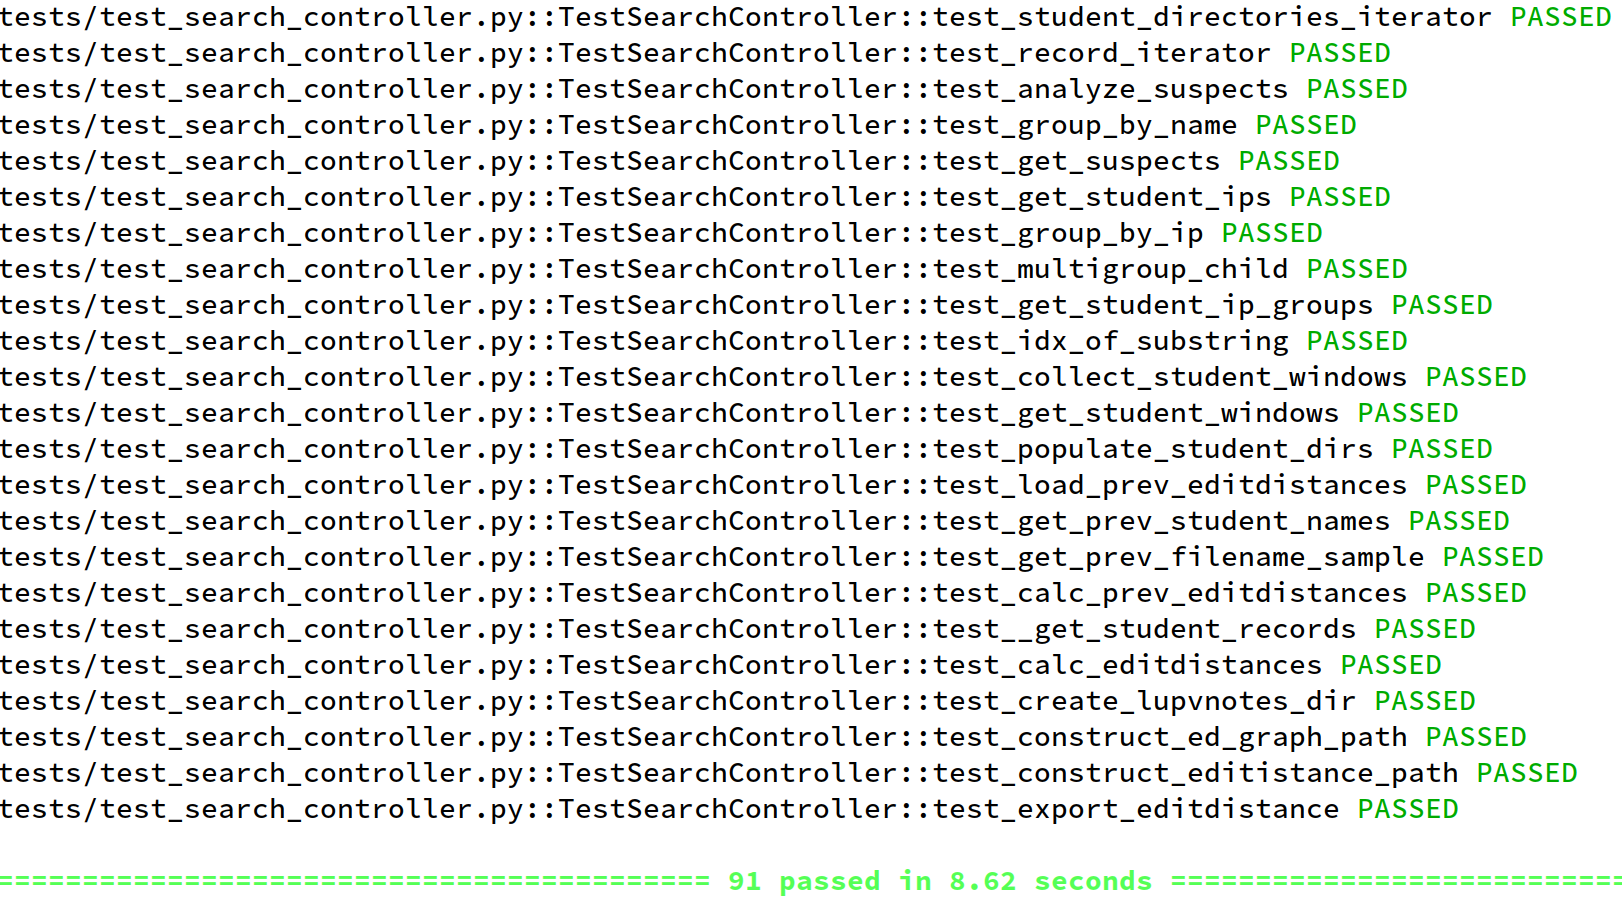
\includegraphics[width=.8\linewidth]{img/automated-test2}
  \caption{Seluruh hasil \emph{automated testing}}
  \label{fig:automated-test}
\end{figure}

\subsection{\emph{Test Script} \emph{Automated Testing} \emph{Class} \emph{Controller}
  \emph{Function} \newline \emph{get\_all\_windows}}

Tabel Kode~\ref{sc:get_all_windows_automated} memaparkan \emph{script}
yang digunakan untuk \emph{automated testing} pada \emph{function
  get\_all\_windows}. Pengujian dilakukan secara terisolasi sehingga
dilakukan \emph{stub} pada proses \emph{Popen}. \emph{Driver} kemudian
memanggil \emph{function get\_all\_windows} dan melakukan
\emph{assert} pada nilai yang dikembalikan.

\par\null\par
\begin{code}
\begin{ignasicblock}[title=get\_all\_windows\_with\_fake,minted language=Python]
def test_get_all_windows_with_fake(self, ctrl, monkeypatch):
  """Test get_all_windows with Fake Object."""
  window_title = b"0x006000ab  0 machine-name foo_window_title"

  def fake_communicate(input=None, timeout=None):
      return window_title, "err"

  Lupr.controllers.controller.Popen = FakePopen
  Lupr.controllers.controller.Popen.communicate = fake_communicate

  output = ctrl.get_all_windows()
  assert output == "foo_window_title\n"
\end{ignasicblock}
  \captionof{listing}{\emph{Test script function}
    get\_all\_windows\_with\_fake}\label{sc:get_all_windows_automated}
\end{code}

\par\null\par
Hasil pengujian \emph{function} \emph{get\_all\_windows} dengan menggunakan
\emph{script} \emph{automated testing} pada Tabel
Kode~\ref{sc:get_all_windows_automated} menghasilkan nilai ``\emph{PASSED}''
seperti yang terlihat pada Gambar~\ref{fig:automated-test}. Maka dapat
dipastikan penggunaan \emph{script automated testing} dapat mempercepat proses
pengujian.

\subsection{\emph{Test Script} \emph{Automated Testing} \emph{Class} \emph{LogController}
  \emph{Function} \emph{populate\_logs}}

Tabel Kode~\ref{sc:populate_logs_automated} memaparkan \emph{script}
yang digunakan untuk \emph{automated testing} pada \emph{function
  populate\_logs}. Pengujian dilakukan secara terisolasi sehingga
dilakukan \emph{stub} pada \emph{function is\_exist} dan \emph{function
  student\_records}. \emph{Driver} kemudian memanggil \emph{function
  populate\_logs} dan melakukan \emph{assert} pada nilai yang
dikembalikan.

\par\null\par
\begin{code}
\begin{ignasicblock}[title=populate\_logs,minted language=Python]
def test_populate_logs_no_records(self, log_ctrl_model):
  """Test populating student logs using dummy data."""
  log_ctrl, log_model = log_ctrl_model
  log_model.student_records = []
  log_model.is_exists = cf.fake_is_exists

  ani_logs = list(
    log_ctrl.populate_logs(
      selected_file="tugas-tif.txt"
    ))

  assert ani_logs == []
\end{ignasicblock}
  \captionof{listing}{\emph{Test script function}
    populate\_logs}\label{sc:populate_logs_automated}
\end{code}

\par\null\par
Hasil pengujian \emph{function} \emph{populate\_logs} dengan menggunakan
\emph{script} \emph{automated testing} pada Tabel
Kode~\ref{sc:populate_logs_automated} menghasilkan nilai ``\emph{PASSED}''
seperti yang terlihat pada Gambar~\ref{fig:automated-test}. Maka dapat
dipastikan penggunaan \emph{script automated testing} dapat mempercepat proses
pengujian.

\subsection{\emph{Test Script} \emph{Automated Testing} \emph{Class} \emph{SearchController}
  \emph{Function} \emph{construct\_ed\_graph\_path}}

Tabel Kode~\ref{sc:construct_ed_graph_path_automated} memaparkan
\emph{script} yang digunakan untuk \emph{automated testing} pada
\emph{function construct\_ed\_graph\_path}. \emph{Function
  construct\_ed\_graph\_path} tidak memanggil \emph{function} lain
sehingga tidak diperlukan adanya \emph{stub}. \emph{Driver} kemudian
memanggil \emph{function construct\_ed\_graph\_path} dan melakukan
\emph{assert} pada nilai yang dikembalikan.

\par\null\par
\begin{code}
\begin{ignasicblock}[title=construct\_ed\_graph\_path,minted language=Python]
def test_construct_ed_graph_path(self, search_ctrl):
  """Test constructing editdistance graph path."""
  graph_path = search_ctrl.construct_ed_graph_path(
    "ani-1111")
  graph_path_2 = search_ctrl.construct_ed_graph_path(
   "ani-1111", "budi-2222")

  assert "/lupv-notes/ani-1111.png" in graph_path
  assert "/lupv-notes/ani-1111_budi-2222.png" in graph_path_2
\end{ignasicblock}
  \captionof{listing}{\emph{Test script function}
    construct\_ed\_graph\_path}\label{sc:construct_ed_graph_path_automated}
\end{code}

\par\null\par
Hasil pengujian \emph{function} \emph{construct\_ed\_graph\_path} dengan
menggunakan \emph{script} \emph{automated testing} pada Tabel
Kode~\ref{sc:construct_ed_graph_path_automated} menghasilkan nilai ``\emph{PASSED}''
seperti yang terlihat pada Gambar~\ref{fig:automated-test}. Maka dapat
dipastikan penggunaan \emph{script automated testing} dapat mempercepat proses
pengujian.

\section{Pengujian \emph{Compatibility}}

Pengujian \emph{compatibility} dilakukan untuk memastikan aplikasi yang dibangun
dapat berjalan dengan baik dan dapat menangani perbedaan format nama
\emph{window} pada enam \emph{desktop environment} utama yang ada pada sistem
operasi \emph{GNU/Linux}. Enam \emph{desktop environment} utama tersebut adalah
\emph{GNOME, KDE, XFCE, Unity, Cinnamon} dan \emph{Phanteon}. Pengujian
\emph{compatibility} pada sistem \emph{Lup Recorder} dilakukan dengan
menjalankan sistem pada seluruh \emph{desktop environment} yang tertera dalam
Tabel~\ref{tab:compatibility-test}, pengujian dilakukan oleh penguji yang
bersangkutan dalam tabel yang sama. Terlihat pada
Tabel~\ref{tab:compatibility-test} sistem juga diujikan terhadap dua
\emph{desktop environment} tambahan yaitu \emph{OpenBox} dan \emph{i3wm}.
Gambar~\ref{fig:compatibility-test} menunjukkan seluruh hasil rekaman sistem
\emph{Lup Recorder} yang dapat dibaca oleh sistem \emph{Lup Viewer}. Hal ini
menandakan bahwa sistem \emph{Lup Viewer} dapat berjalan dengan baik pada
seluruh \emph{desktop environment} dalam
Tabel~\ref{tab:compatibility-test}. Pengujian sistem \emph{Lup Viewer} dilakukan
dengan menjalankannya pada \emph{desktop environment} yang
berbeda-beda. Gambar~\ref{fig:compatibility-i3wm} menunjukkan sistem \emph{Lup
  Viewer} dapat berjalan dengan baik pada \emph{desktop environment i3wm} dan
Gambar~\ref{fig:compatibility-xfce} menunjukkan sistem \emph{Lup Viewer}
berjalan dengan baik pada \emph{desktop environment XFCE}.

{\makegapedcells
  \begin{longtable}{|c|L{4.5cm}|c|L{1cm}|}
    \caption{Daftar \emph{desktop environment} yang diuji} \label{tab:compatibility-test}\\
    \hline
    \thead{No} & \thead{Nama Penguji} & \thead{\emph{Desktop} \\ Environment} & \thead{Versi} \\\hline
    \endfirsthead
    \hline
    \thead{No} & \thead{Nama Penguji} & \thead{\emph{Desktop} \\ Environment} & \thead{Versi} \\\hline
    \endhead
    %
    1 & Bintang Dimas PAR & \emph{GNOME} & 3.28.2 \\\hline
    2 & Muhammad Iqbal K & \emph{GNOME} & 3.28.2 \\\hline
    3 & Laode Muhamad Fauzan & \emph{KDE} & 5.9.15 \\\hline
    4 & Husein Abdulbar  & \emph{KDE} & 5.15.5 \\\hline
    5 & Rofy Firmansyah R & \emph{KDE} & 5.15.5 \\\hline
    6 & Satria Adhi Kharisma & \emph{XFCE} & 4.12 \\\hline
    7 & Dese Narfa Firmansyah & \emph{XFCE} & 4.12 \\\hline
    8 & Rizaldy Firmansyah Y & \emph{Unity} & 7 \\\hline
    9 & Insan Nurzaman  & \emph{Cinnamon} & 3.6.6 \\\hline
    10 & Jerna Ferda Kusuma & \emph{Cinnamon} & 4.0.10 \\\hline
    11 & Rahmat Guntur Husodo & \emph{Cinnamon} & 4.0.10 \\\hline
    12 & Febristya AF  & \emph{Pantheon} &  5.0 \\\hline
    13 & Achmad Rizki Aditama & \emph{OpenBox} & 3.6.1 \\\hline
    14 & Mohammad Anton RS & \emph{i3wm} & 4.16.1 \\\hline
  \end{longtable}
}

\begin{figure}[tph]
  \centering
  %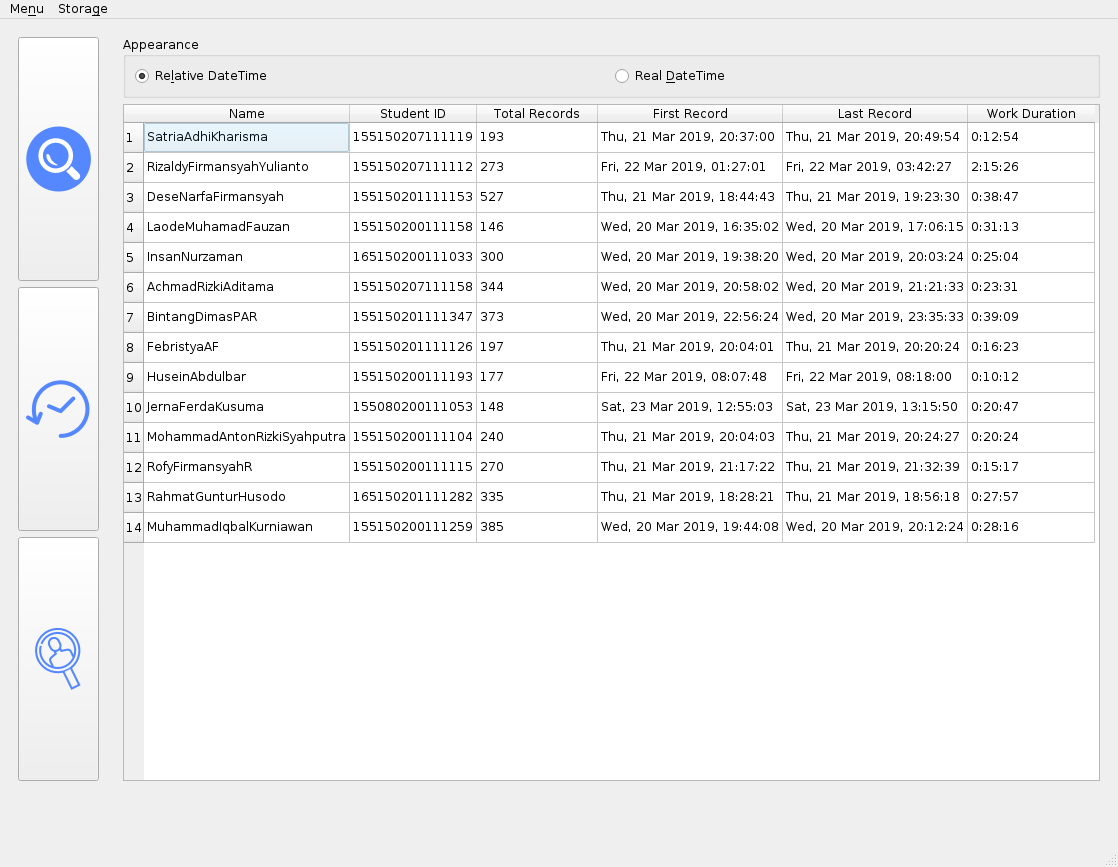
\includegraphics[width=.9\linewidth]{img/compatibility-res1}
  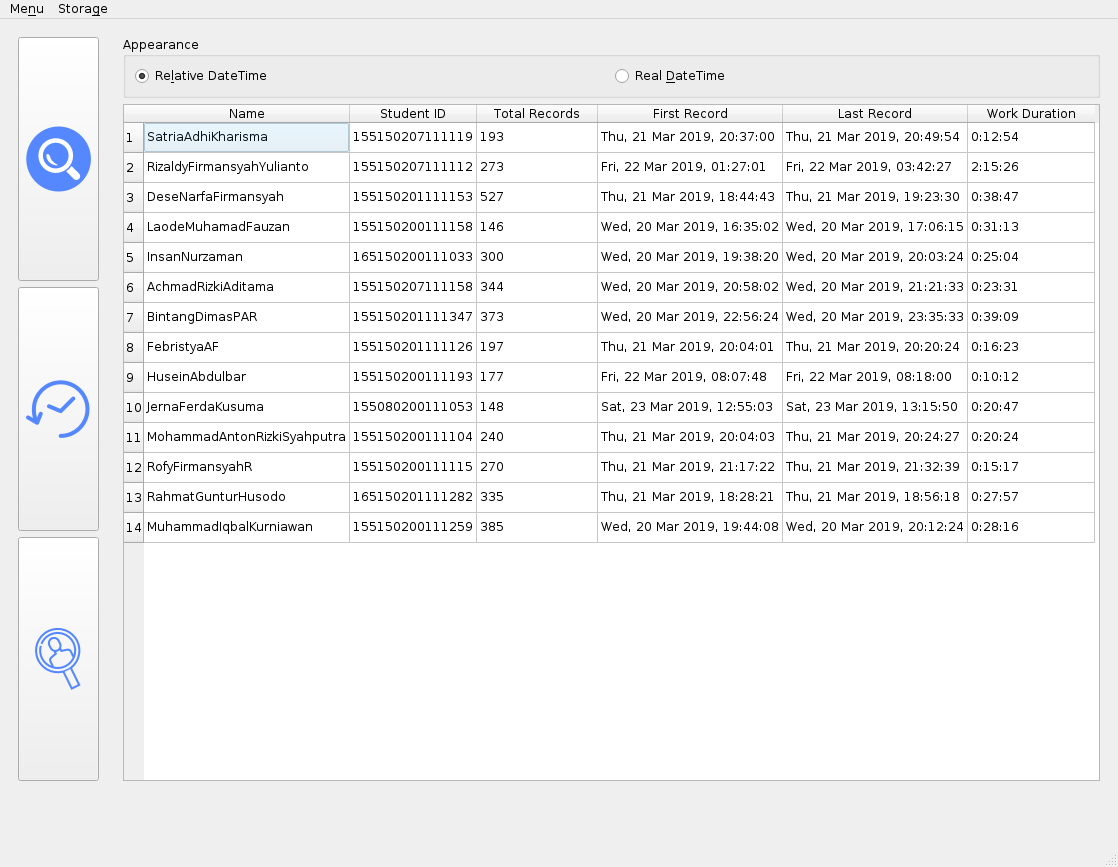
\includegraphics[angle=90,width=1.1\linewidth]{img/compatibility-res1}
  \caption{Sistem \emph{Lup Recorder} berhasil merekam berkas tugas pada \emph{desktop environment} yang berbeda-beda}
  \label{fig:compatibility-test}
\end{figure}

\begin{figure}[tph]
  \centering
  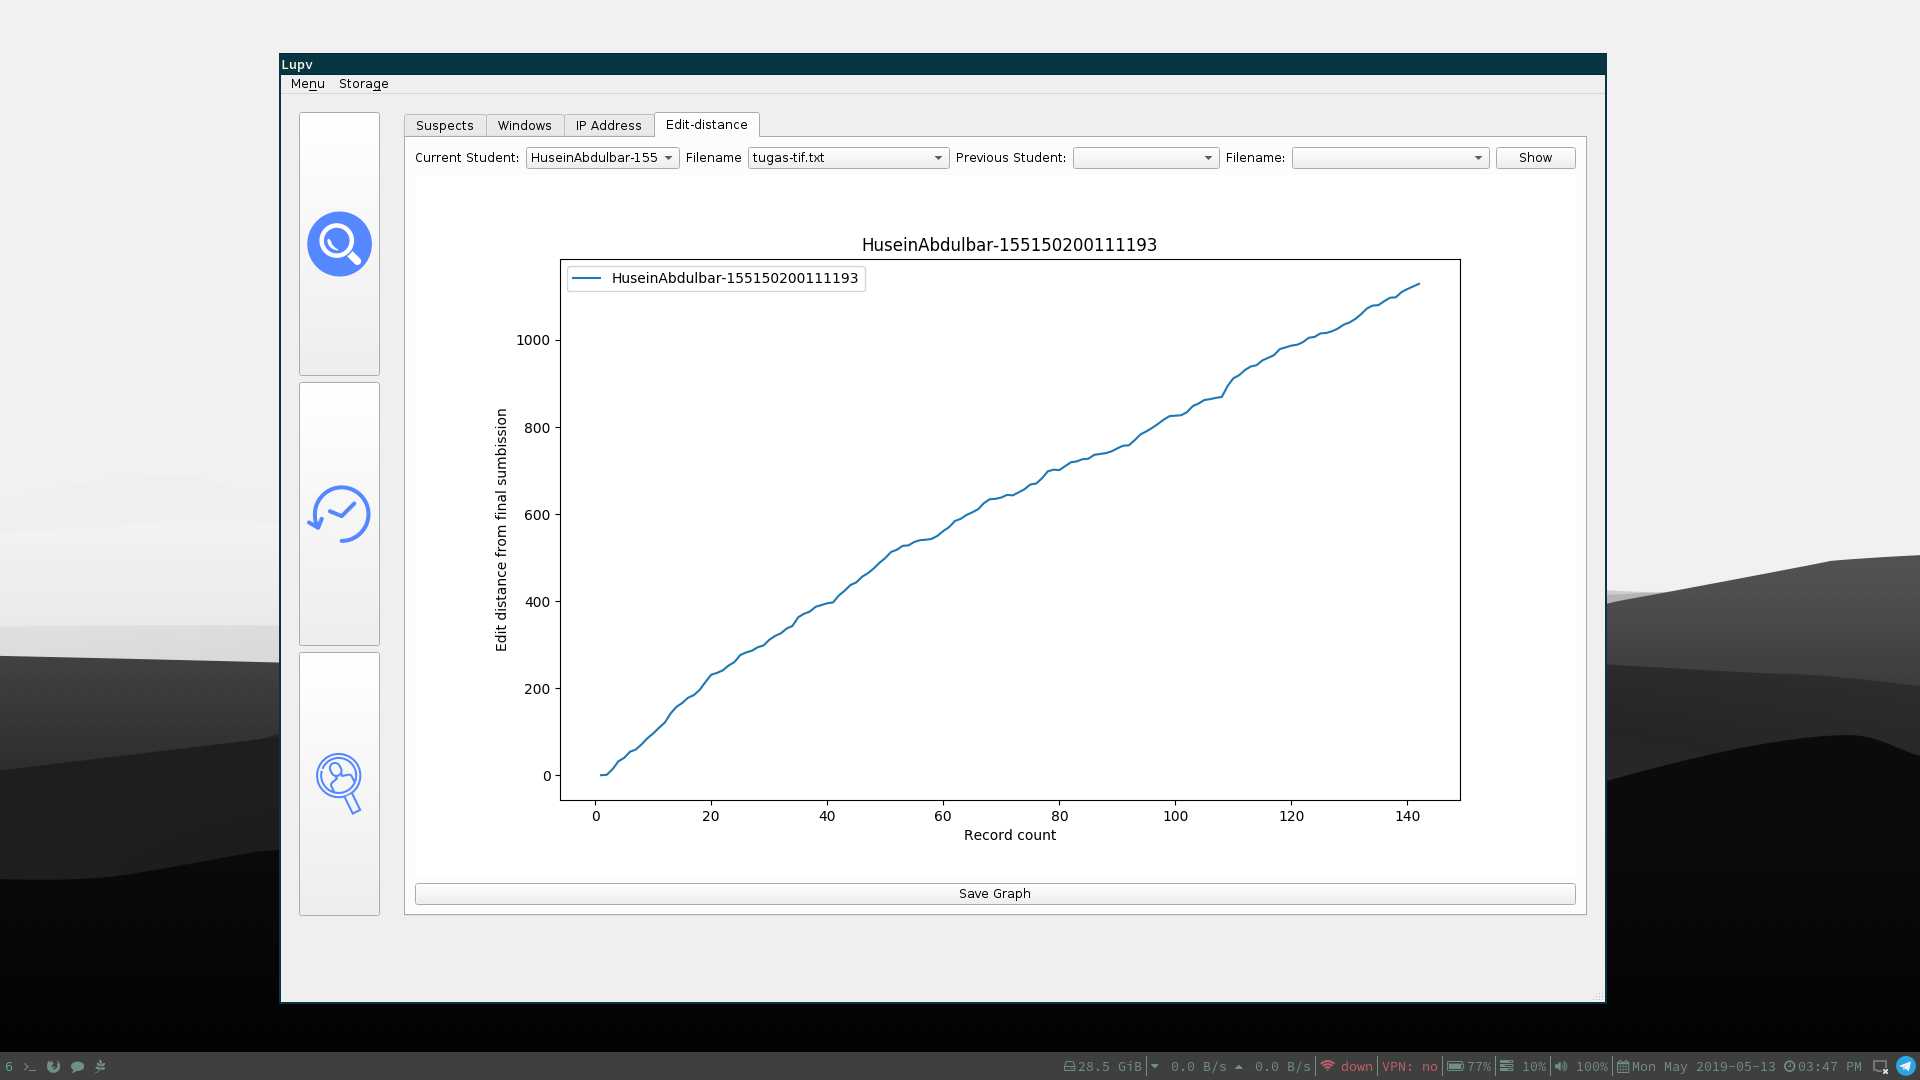
\includegraphics[width=.9\linewidth]{img/compatibility-i3wm}
  \caption{\emph{Lup Viewer} pada \emph{desktop environment i3wm}}
  \label{fig:compatibility-i3wm}
\end{figure}

\begin{figure}[tph]
  \centering
  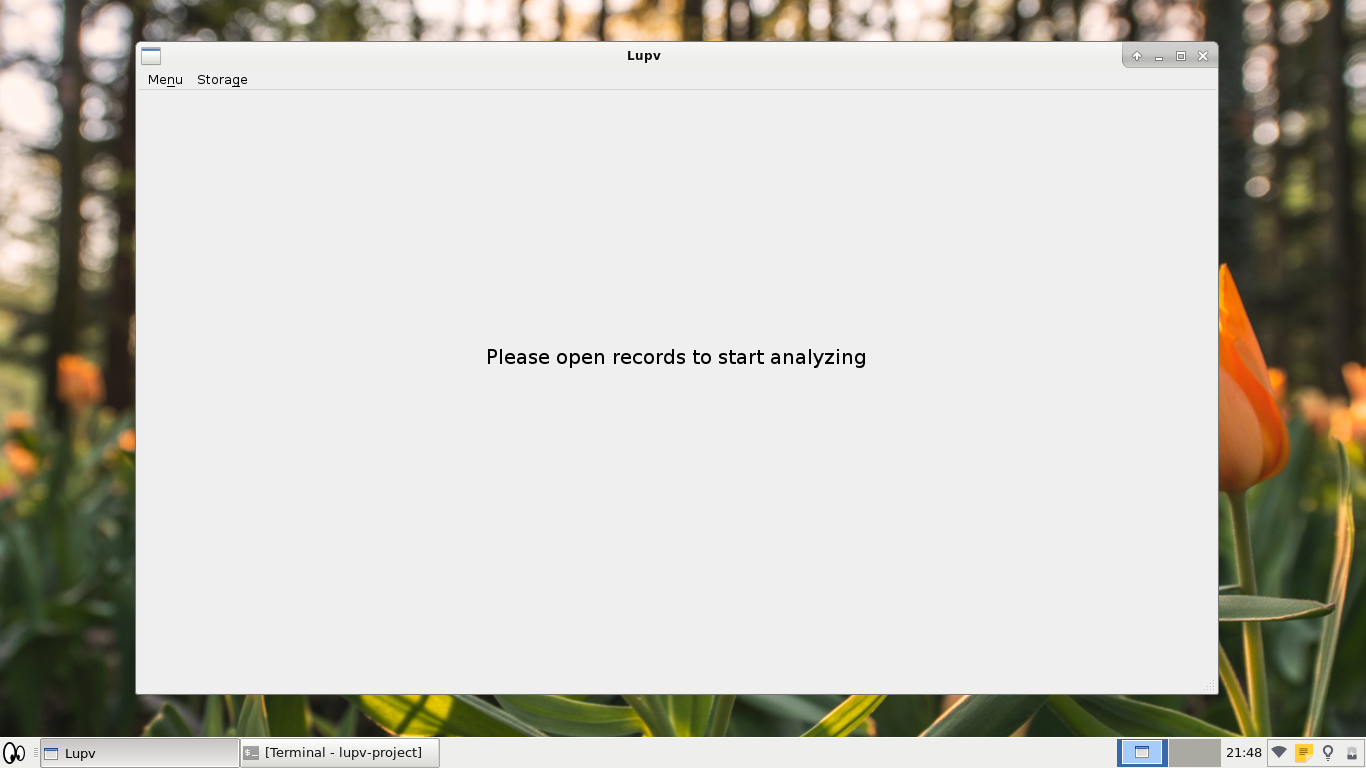
\includegraphics[width=.9\linewidth]{img/compatibility-xfce}
  \caption{\emph{Lup Viewer} pada \emph{desktop environment XFCE}}
  \label{fig:compatibility-xfce}
\end{figure}

%%% Local Variables:
%%% coding: utf-8
%%% mode: latex
%%% TeX-engine: xetex
%%% TeX-master: "skripsi"
%%% ispell-local-dictionary: "id"
%%% End:
